%% 
%% This is a sample doctoral dissertation.  It shows the appropriate
%% structure for your dissertation.  It should handle most of the
%% strange requirements imposed by the Grad school; like the different
%% handling of titles of one/many appendices.  It will automatically
%% handle the linespacing changes.  The body default is double-spaced
%% (except when you use the singlespace or condensed options).  The
%% default for quotations is single-space, and the default for tabular
%% environments is also single-space.  
%%
%% This class adds the following commands and environments to the
%% report class, upon which it is based:
%% Commands
%% ------------
%% \degree{name}{abbrv} -- Sets the name and abbreviation for the degree.
%%                         These default to ``Doctor of Philosopy''
%%                         and ``Ph.D.'', respectively.
%% \copyrightyear{year} -- for the copyright page.
%% \bachelors{degree}{institution} -- for the abstract
%% \masters{degree}{institution}   --  "
%%     if you have other degrees you may use
%% \secondbachelors{degree}{institution}
%% \thirdbachelors{degree}{institution}
%% \secondmasters{degree}{institution}
%% \thirdmasters{degree}{institution}
%% \priordoctorate{degree}{institution}
%%
%% \committeechair{name}           -- for the signature page
%% or, if you have two co-chairs:
%% \cochairs{first name}{second name}
%%
%% \firstreader{name}              --  "
%% \secondreader{name}             --  "
%% \thirdreader{name}              -- (optional)
%% \fourthreader{name}             --  "
%% \fifthreader{name}              --  "
%% \sixthreader{name}              --  "
%% \departmentchair{name}          -- for the signature page
%% \departmentname{name}           --  "
%%
%% \copyrightpage                  -- produces the copyright page
%% \signaturepage                  -- produces the signature page
%%
%% \frontmatter                    -- these are required in their various
%% \mainmatter                     -- appropriate locations
%% \backmatter                     --
%%
%% \unnumberedchapter[toc]{name}   -- like \chapter, except that it
%%                                    produces an unnumbered chapter;
%%                                    alternatively, like \chapter*,
%%                                    except that it lists the chapter
%%                                    in the table of contents.
%%
%% New environments:
%%   dedication  -- for the dedication
%%   abstract    -- for the abstract
%%
%% The thesis documentclass is built on top of the report document class.
%% It accepts all of the options that the report class accepts, plus the
%% following:
%%     doublespace -- the default, indicates double spacing as per U.Mass.
%%                    requirements.  You will need this when you do your
%%                    final copy.
%%     singlespace -- for earlier work, not acceptable to the Grad school
%%     condensed   -- for earlier work, not acceptable to the Grad school,
%%                    creates condensed versions of the frontmatter. 
%%                    Condensed implies singlespace.
%%     dissertation - the default, indicates that this document is a
%%                    dissertation.
%%     proposal    -- indicates that this document is a dissertation proposal,
%%                    rather than a dissertation.  This will only change the
%%                    wording on the title and signature pages.
%%     thesis      -- indicates that this document is a Master's thesis 
%%                    rather than a doctoral dissertation.  This also changes
%%                    the default for \degree to Master of Science, M.S.
%%     allowlisthypenation -- (the default), allows hyphenation of words in
%%                    the table of contents, the list of figures, and the list
%%                    of tables.  I believe that this is acceptable to the 
%%                    Graduate School.
%%     nolisthyphenation -- disallows hyphenation of words in the table of
%%                    contents and the list of figures and tables.  Use this 
%%                    option if the Grad School doesn't like your hyphenation.
%%     nicerdraft  -- relaxes some of the Grad School's rules for working with
%%                    drafts -- has no effect when doublespace is in effect
%%     nonicerdraft -- the default, leaves things in draft as they will be in
%%                     the final version
%% umassthesis changes the default font size to 12pt, but you may specify 10pt or
%%   11pt in the options.
\documentclass{umassthesis}          % for Ph.D. dissertation or proposal
\usepackage[hidelinks]{hyperref}
\usepackage{graphicx}
\usepackage{booktabs}
\usepackage{multirow}
\usepackage{soul}

\usepackage[style=apa, backend=biber]{biblatex}
\addbibresource{Papers.bib}
% \documentclass[thesis]{umassthesis}  % for Master's thesis

%%
%% If you have enough figures or tables that you run out of space for their
%% numbers in the List of Tables or List of figures, you can use the following
%% command to adjust the space left for numbers.  The default is shown:
%%
%% \setlength{\tablenumberwidth}{2.3em}

%% Use the hyperref package if you're producing a version for online
%% distribution and you want hyperlinks.  Note that the Grad School doesn't want
%% their PDF viewers to colorize or otherwise highlight the links; use the
%% hidelinks option to hyperref to avoid decorating links.
%\usepackage[hidelinks]{hyperref}

%% One way of formatting the epigraph/frontispiece is to use this package.
%\usepackage{epigraph}

\begin{document}

%%
%% You must fill in all of these appropriately
\title{Context dependence in perceptual and preferential choice}
\author{Sean Patrick Conway}
\date{September 2025} % The date you'll actually graduate -- must be
                     % February, May, or September
\copyrightyear{2025}

\committeechair{Andrew L. Cohen}
\firstreader{Youngbin Kwak}
\secondreader{Elizabeth Miller}
\thirdreader{Jeffrey Starns}

\departmentchair[Department Chair]{Ilia Karatsoreos} 
\departmentname{Psychological and Brain Sciences}

\degree{Doctor of Philosopy}

%%
%% These lines produce the title, copyright, and signature pages.
%% They are Mandatory; except that you could leave out the copyright page
%% if you were preparing an M.S. thesis instead of a PhD dissertation.
\frontmatter
\maketitle
\copyrightpage     %% not required for an M.S. thesis
\signaturepage

%%
%% Dedication is optional -- but this is how you create it
%\begin{dedication}              % Dedication page
%  \begin{center}
%    \emph{To those little lost sheep.}
%  \end{center}
%\end{dedication}

%%
%% Epigraph (aka frontispiece) is also optional, but this is one way you
%% can create it
%\begin{frontispiece}
%  %% Format to your liking -- see documentation of epigraph package
%  \setlength{\epigraphrule}{0pt}
%
%  \begin{epigraphs}
%    \qitem{%
%      \itshape
%      Mary had a little lamb,\\
%      Her fleece was white as snow.\\
%      \vspace{\baselineskip}
%      And everywhere that Mary went\\
%      The lamb was sure to go.
%      \vspace{\baselineskip}}
%    {Sarah Josepha Hale}
%
%    \vspace{2\baselineskip}
%    \qitem{%
%      \itshape
%      Baa, baa, black sheep,\\
%      Have you any wool?\\
%      Yes, sir, yes, sir,\\
%      Three bags full;\\
%      One for the master,\\
%      And one for the dame,\\
%      And one for the little boy\\
%      Who lives down the lane.
%      \vspace{\baselineskip}}
%    {English Nursery Rhyme}
%
%  \end{epigraphs}
%\end{frontispiece}

%%
%% Acknowledgements are optional...yeah, right.
\chapter{Acknowledgments}             % Acknowledgements page
Thank you to...

%%
%% Abstract is MANDATORY. -- Except for MS theses
\begin{abstract}                % Abstract

\end{abstract}

%%
%% Preface goes here...would be just like Acknowledgements -- optional
%% \chapter{Preface} 
%% ...


%%
%% Table of contents is mandatory, lists of tables and figures are 
%% mandatory if you have any tables or figures; must be in this order.
\tableofcontents                % Table of contents
\listoftables                   % List of Tables
\listoffigures                  % List of Figures

%%
%% I don't handle List of Abbreviations
%% I don't handle Glossary

%%%%%%%%%%%%%%%%%%%%%%%%%%%%%%%%%%%%%%%%%%%%%%%%%%%%%%%%%%%%%%%%%%%%%%%%%
%% Time for the body of the dissertation
\mainmatter   %% <-- This line is mandatory

%%
%% If you want an introduction, which is not a numbered chapter, insert
%% the following two lines.  This is OPTIONAL:
%\unnumberedchapter{Introduction}


%%
%% Some sample text
\chapter{Introduction}

\subsection{Overview}

One known fact about human decision-making is that context can affect people's choices. That is, the relative likelihood of choosing one option over another can vary systematically with the menu of options, the \textit{choice set}. These findings are known as \textit{context effects}. One notable context effect, the attraction effect, occurs when the choice share of a \textit{target} option is boosted upon the inclusion of a similar but inferior \textit{decoy} option. Another finding, the repulsion effect, occurs when a decoy boosts the choice share of a \textit{dissimilar} option, known as the \textit{competitor}, rather than the target.

The attraction and repulsion effects, originally studied in preferential choice, have recently been shown to occur in simple perceptual decision-making \parencite{trueblood2013not,spektorWhenGoodLooks2018b}. This is theoretically interesting because it suggests that context effects are a theoretical primitive rather than a feature of high-level choice \parencite{trueblood2013not}. The goal of this research is to understand how and why these effects occur by employing well-studied statistical models from the psychology and economics literature. 

This dissertation is structured as follows. In Chapter 1, I introduce the relevant empirical and theoretical literature in context effects. The goal of Chapter 2 is to develop and test a statistical model of perceptual variability when applied to context effects. In Experiment 1, I first show that the types of stimuli used in perceptual choice context effects experiments are easily confusable and vary systematically with theoretically relevant properties of the stimuli. In Experiment 2, I use the results of a high-powered psychophysics experiment to show that the repulsion effect, but not the attraction effect, is naturally predicted by this statistical model due to the fact that pairs of similar stimuli are more strongly perceptually correlated than pairs of dissimilar stimuli. In Chapter 3, I further test the statistical model by applying it to best-worst choice. In Chapter 4, I generalize the model to preferential choice. 

\subsection{Introducing the Attraction Effect}

In decision-making experiments, researchers present participants with a finite set of options on each trial and ask them to select a single option. Researchers universally assume that participants use the input they receive (i.e., the value of each option) to arrive at a choice. The study of choice spans multiple fields, including psychology, economics, marketing, and political science. In economics, for example, researchers have developed models based on the idea that, while preferences may vary from moment to moment, people generally make rational choices in any given choice setting \parencite{mcfadden2001economic}. In psychology and marketing, however, researchers have identified a set of phenomena that violate such assumptions, by showing that choices vary based on the \textit{choice set}, or the menu of available options. This class of phenomena is known as \textit{context effects} \parencite{adler2024forty}.

Context effects are interesting to decision-making researchers because they violate properties of large classes of choice models, such as Independence of Irrelevant Alternatives (IIA) \parencite{ray1973independence} and regularity \parencite{mcfadden2001economic}. Psychologists have developed numerous cognitive process models to explain how context effects can arise \parencite{roeMultialternativeDecisionField2001a,usherLossAversionInhibition2004a,truebloodMultiattributeLinearBallistic,wollschlager2NaryChoiceTree2012a,bergnerVAMPVotingAgent2019b,noguchiMultialternativeDecisionSampling2018a,bhatiaAssociationsAccumulationPreference2013b,tversky1993context}. These models vary considerably in their mechanisms but align in the common assumption that decision makers take in the veridical values of each option on each attribute and use these values to arrive at a preference state, leading to a decision. 

This dissertation will explore context effects in both perceptual and preferential decision-making. In particular, I will explore the attraction effect and its reversal, the repulsion effect. I summarize these effects and the relevant literature below.

To begin, I first demonstrate a notable context effect, the \textit{attraction effect}. As a demonstration, see \ref{fig:fig_opts} (left panel), which shows a graphical configuration of various choice options. These options vary on two dimensions (or attributes), where higher values of an attribute are always preferred. I give these dimensions generic names to emphasize that they may be anything from the fuel efficiency and horsepower of cars in a consumer choice experiment to the height and width of rectangles in a perceptual choice experiment.

\begin{figure}
  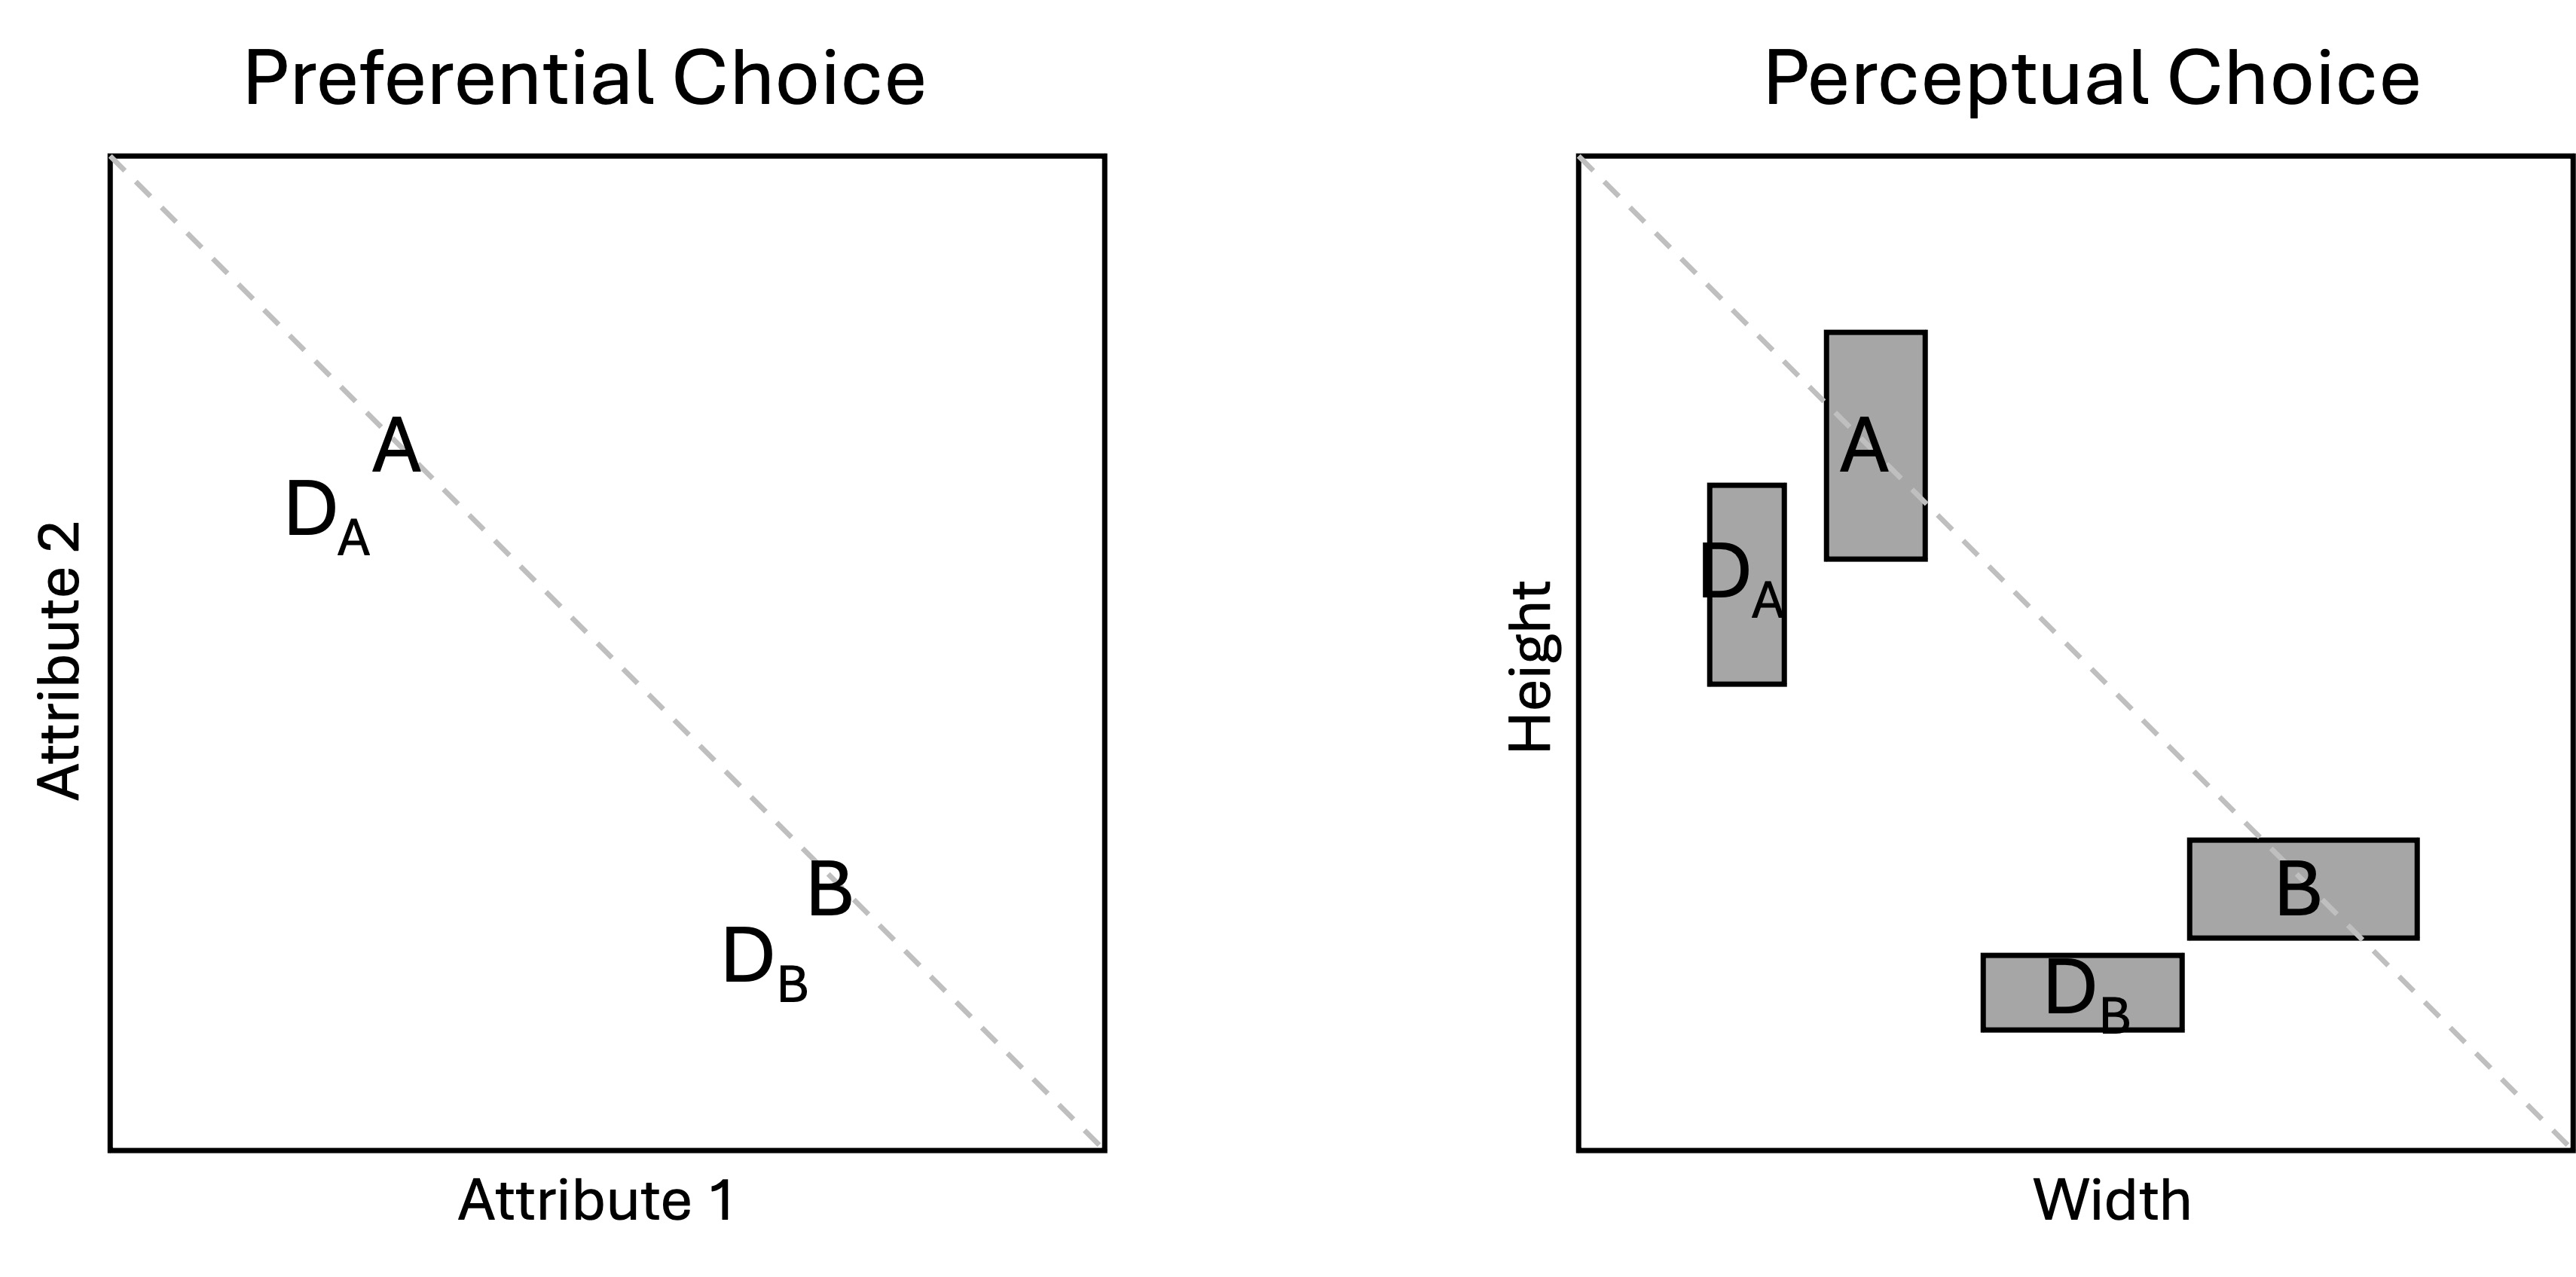
\includegraphics[width=\linewidth]{figures/pref_v_percep.jpg}
  \caption{A graphical depiction of choice options in the attraction/repulsion effect. Left panel: preferential choice. Right panel: perceptual choice.}
  \label{fig:fig_opts}
\end{figure}

In Figure \ref{fig:fig_opts} (left panel), options $A$ and $B$ trade off on attributes. $A$ is high on dimension 2 but low on dimension 1, while $B$ is high on dimension 1 but low on dimension 2. A decision-maker who assigns equal importance to both dimensions should be indifferent between both options when presented with choice set $[A,B]$. Now, however, consider option $D_{A}$, which is inferior to $A$ and $B$, but more similar to $A$ than to $B$\footnote{Similarity here is negatively related to distance in attribute space \parencite{shepardUniversalLawGeneralization1987c}.}. Similarly, $D_{B}$ is inferior to both $A$ and $B$ but more similar to $B$. The attraction effect is the finding that choice for $A$ over $B$ is greater given set ${A,B,D_{A}}$ then given set $A,B,D_{B}$\footnote{This is the weak version of the attraction effect. A strong version requires the ordering of P(A) and P(B) to change with choice set. See \textcite{davis2023illustrated} for a discussion of similar issues.}. 
Choice models often, though not necessarily, assume the \textit{Independence of Irrelevant Alternatives}(IIA) principle. IIA states that the relative likelihood of choosing a particular option over another is invariant of the choice set \parencite{ray1973independence}.  To demonstrate, let $A$, $B$, $D_{A}$, and $D_{B}$ be discrete choice options, $[]$ denote the options in a choice set, and $P(A|[A,B])$ denote the probability of choosing option $A$ from a set consisting of $A$ and $B$. According to IIA:

\begin{align}
  \frac{P(A|[A,B,D_{A}])}{P(B|[A,B,D_{A}]}=\frac{P(A|[A,B,D_{B}])}{P(B|[A,B,D_{B}]}
  \label{eqn:iia}
\end{align}

However, in the attraction effect:

\begin{align}
  \frac{P(A|[A,B,D_{A}])}{P(B|[A,B,D_{A}]}>\frac{P(A|[A,B,D_{B}])}{P(B|[A,B,D_{B}]}
  \label{eqn:iia_att}
\end{align}

Thus, IIA is violated.

In the context effects literature, it is common to refer to the similar, dominated option as \textit{decoy}, the similar dominating option as a \textit{target}, and the dissimilar dominating option as a \textit{competitor}. I adopt this terminology through this dissertation. For example, in the choice set $[A,B,D_{A}]$, $A$ is the target, $B$ is the competitor, and $D_{A}$ is the decoy.  The decoy is dominated by the target, so no rational agent should intentionally select it over the target.  

The attraction effect was first demonstrated by \textcite{huberAddingAsymmetricallyDominated1982d}\footnote{These authors referred to this finding as the asymmetric dominance effect. To stay consistent with contemporary research, I use the term attraction effect throughout this dissertation.}, who tested participants with duples and triples of choice options, using products such as cars, beers, and TV sets. The authors showed that the introduction of an asymmetrically dominated decoy tended to increase the choice share of a similar, target option. Such a result violates IIA but also a principle known as regularity, which states that the introduction of another option to a choice set cannot increase the probability of choosing any given option (CITE COLONIUS 1984, MACKAY AND ZINNES 1995, MARLEY 1989). That is to say:

\begin{align}
  P(A|[A,B])\geqP(A|A,B.D_{A})
  \label{eqn:reg_att}
\end{align}

Thus, \textcite{huberAddingAsymmetricallyDominated1982d}'s finding that $P(A|[A,B])\leqP(A|A,B.D_{A})$ violates this assumption. \textcite{huber1983market} replicated these results and also showed that if the decoy has a relatively high value, it can actually take choice shares away from the target. This result suggests that the relative positioning of the decoy to the target can greatly affect patterns of choice, a finding explored by numerous other researchers which has strong theoretical consequences (see below). 

Numerous researchers have since demonstrated the attraction effect in preferential choice, including in real-world scenarios. \textcite{doyleRobustnessAsymmetricallyDominated1999} found an attraction effect in real world supermarket choices by adding a decoy option to an existing product set, where the decoy option was the same brand and price as the target, but of a lower volume. \textcite{van2021attract} showed that the attraction effect can be used to induce people to choose healthier food items. \textcite{slaughterDecoyEffectsAttributelevel1999b} showed that the attraction effect can be found even without the explicit attribute descriptions commonly used in laboratory experiments, when participants must infer option attributes. 

Context effects like the attraction effect have strong theoretical implications. Traditional models of choice, as used in economics and marketing research \parencite{mcfadden2001economic}, treat the \textit{utility}, or value, of each option as a random variable whose parameters are to be estimated from choice data, and on each trial of a choice experiment the participant samples values from these distribution and deterministically chooses the option with the highest sampled value. These models are known as \textit{Random Utility Models} (RUMs). When utilities are assumed to follow Type 1 Generalized Extreme Value distribution, the logit or softmax model is used (CITE). As will be the focus of much of this dissertation, the probit model assumes Gaussian distributed utilities (CITE). Often (though not necessarily) RUMs assume IIA, though this assumption can be relaxed by assuming set or alternative specific intercepts (CITE) or allowing correlations between options and/or attributes (CITE). \textcite{haaijer1998utility} showed that the probit model shows an improved fit to context effect data by allowing such correlations. I elaborate on this class of models below. 

In cognitive psychology, researchers have developed cognitive process models that attempt to explain the cognitive processes that lead to context effects \parencite{truebloodMultiattributeLinearBallistic,roeMultialternativeDecisionField2001a,usherLossAversionInhibition2004a,bhatiaAssociationsAccumulationPreference2013b,noguchiMultialternativeDecisionSampling2018a,wollschlager2NaryChoiceTree2012a,bergnerVAMPVotingAgent2019b,tverskyEliminationAspectsTheory1972,tversky1993context}. These models differ, to varying degrees, in their explanations for the attraction effect. Many, however, rely on comparisons between the target and the similar, but inferior, decoy, which boost an internal  preference state for the target. \textcite{roeMultialternativeDecisionField2001a}'s Multialternative Decision Field Theory (MDFT) model proposes that the similarity between target and decoy causes frequent target-decoy comparisons, and through a lateral inhibition, the negative valence for the decoy causes a boost to the preference state of the target at the expense of the competitor. \textcite{truebloodMultiattributeLinearBallistic}'s Multiattribute Linear Ballistic Accumulator (MLBA) model proposes that pairwise attention weights, which are a function of the similarity between options, increase the importance of target-decoy comparisons and thus boost preference for the target. 

This dissertation does not explore the predictive success of these models, nor does it incorporate model fitting to compare these models. Indeed, other researchers have done such analyses \parencite{turnerCompetingTheoriesMultialternative2018a,cataldoModelingPreferenceReversals2021,evansResponsetimeDataProvide2019b,molloyWhatResponseTime2019a,berkowitschRigorouslyTestingMultialternative2014b}. Instead, I use behavioral experiments and statistical modeling to understand how context dependence arises in various domains.

The attraction effect is not limited to merely consumer choice. Researchers have found the attraction effect in risky choice \parencite{mohr2017attraction}, policy choice \parencite{herneDecoyAlternativesPolicy1997b}, intertemporal choice \parencite{mariniAttractionComesMany2020}, probability judgment \parencite{caiWhenAlternativeHypotheses2023}, medical decision-making \parencite{schwartz1999more}, charitable donation \parencite{pittarello2020three},  inference \parencite{truebloodMultialternativeContextEffects2012}, job candidate selection \parencite{highhouseContextDependentSelectionEffects1996}, political choice \parencite{pan1995attractiovoting}, and, as will be the focus of much of this dissertation, perceptual choice \parencite{evansImpactPresentationOrder2021,trueblood2013not,spektorRepulsionEffectPreferential2022,spektorWhenGoodLooks2018b,yearsleyContextEffectsSimilarity2022,turnerCompetingTheoriesMultialternative2018a,liaoInfluenceDistanceDecoy2021}. 

\subsection{From preferential to perceptual choice}

As mentioned above, researchers have begun studying context effects in perceptual choice. \textcite{trueblood2013not} demonstrated the attraction effect in perceptual choice. In their experiments, participants saw three rectangles on each trial, arranged in a horizontal array, and they selected the option they believed to have the largest area. As a demonstration of this stimulus configuration, see \ref{fig:fig_opts} (right panel).  Options $A$ and $B$ have equal area but trade off in height and width. \footnote{\textcite{trueblood2013not} also demonstrated the similarity and compromise effects.} Notably, the title of their paper was "Not Just for Consumers: Context Effects Are Fundamental to Decision Making", and in their General Discussion, \textcite{trueblood2013not} argued "our experiments suggest that these context effects are a general feature of human choice behavior because they are a fundamental part of decision-making processes. As such, our results challenge explanations of these effects exclusively in terms that are unique to high-level decision making and thus call for a common theoretical explanation that applies across paradigms." (p. 907). According to \textcite{trueblood2013not}, context effects are not idiosyncratic to high-level choices but are a fundamental part of the choice process. \textcite{trueblood2013not} also used these perceptual results to argue against the context-dependent advantage (CDA) model developed by \textcite{tversky1993} as well as the Leaky Competing Accumulators model of \textcite{usherLossAversionInhibition2004a}, as these models use "loss aversion" (i.e., the idea that an option's disadvantages on an attribute are weighted more strongly than its advantages on other attributes) to account for context effects. 

\textcite{turnerCompetingTheoriesMultialternative2018a} replicated \textcite{trueblood2013not}'s results and performed a large scale modeling study. The authors compared the ability of numerous mechanisms assumed by decision models to account for context effects. For example, \textcite{turnerCompetingTheoriesMultialternative2018a} concluded that pairwise comparisons on individual attributes greatly improves models' ability to account for context effects. This may not be appropriate, however, given a perceptual domain where dimensions may not be separable \parencite{ashbyVarietiesPerceptualIndependence1986a}. 

\textcite{spektorWhenGoodLooks2018b} followed up on this work and demonstrated the \textit{repulsion effect} in a rectangle choice experiment. In the repulsion effect, the competitor's choice share is higher than the target's choice share \parencite{liaoInfluenceDistanceDecoy2021,evansImpactPresentationOrder2021,simonsonVicesVirtuesMisguided2014,frederickLimitsAttraction2014b,spektorRepulsionEffectPreferential2022,banerjeeFactorsThatPromote2024,bhui2021rational}. In \textcite{spektorWhenGoodLooks2018b}'s experiments, the target and competitor options varied in area, such that one option was always larger, but on average they were the same size. The researchers also varied the \textit{target-decoy attribute distance} (TDD), the percentage difference between the target and decoy areas. For example, if TDD is $2\%$, the decoy is $2\%$ smaller than the target. 

\begin{figure}
   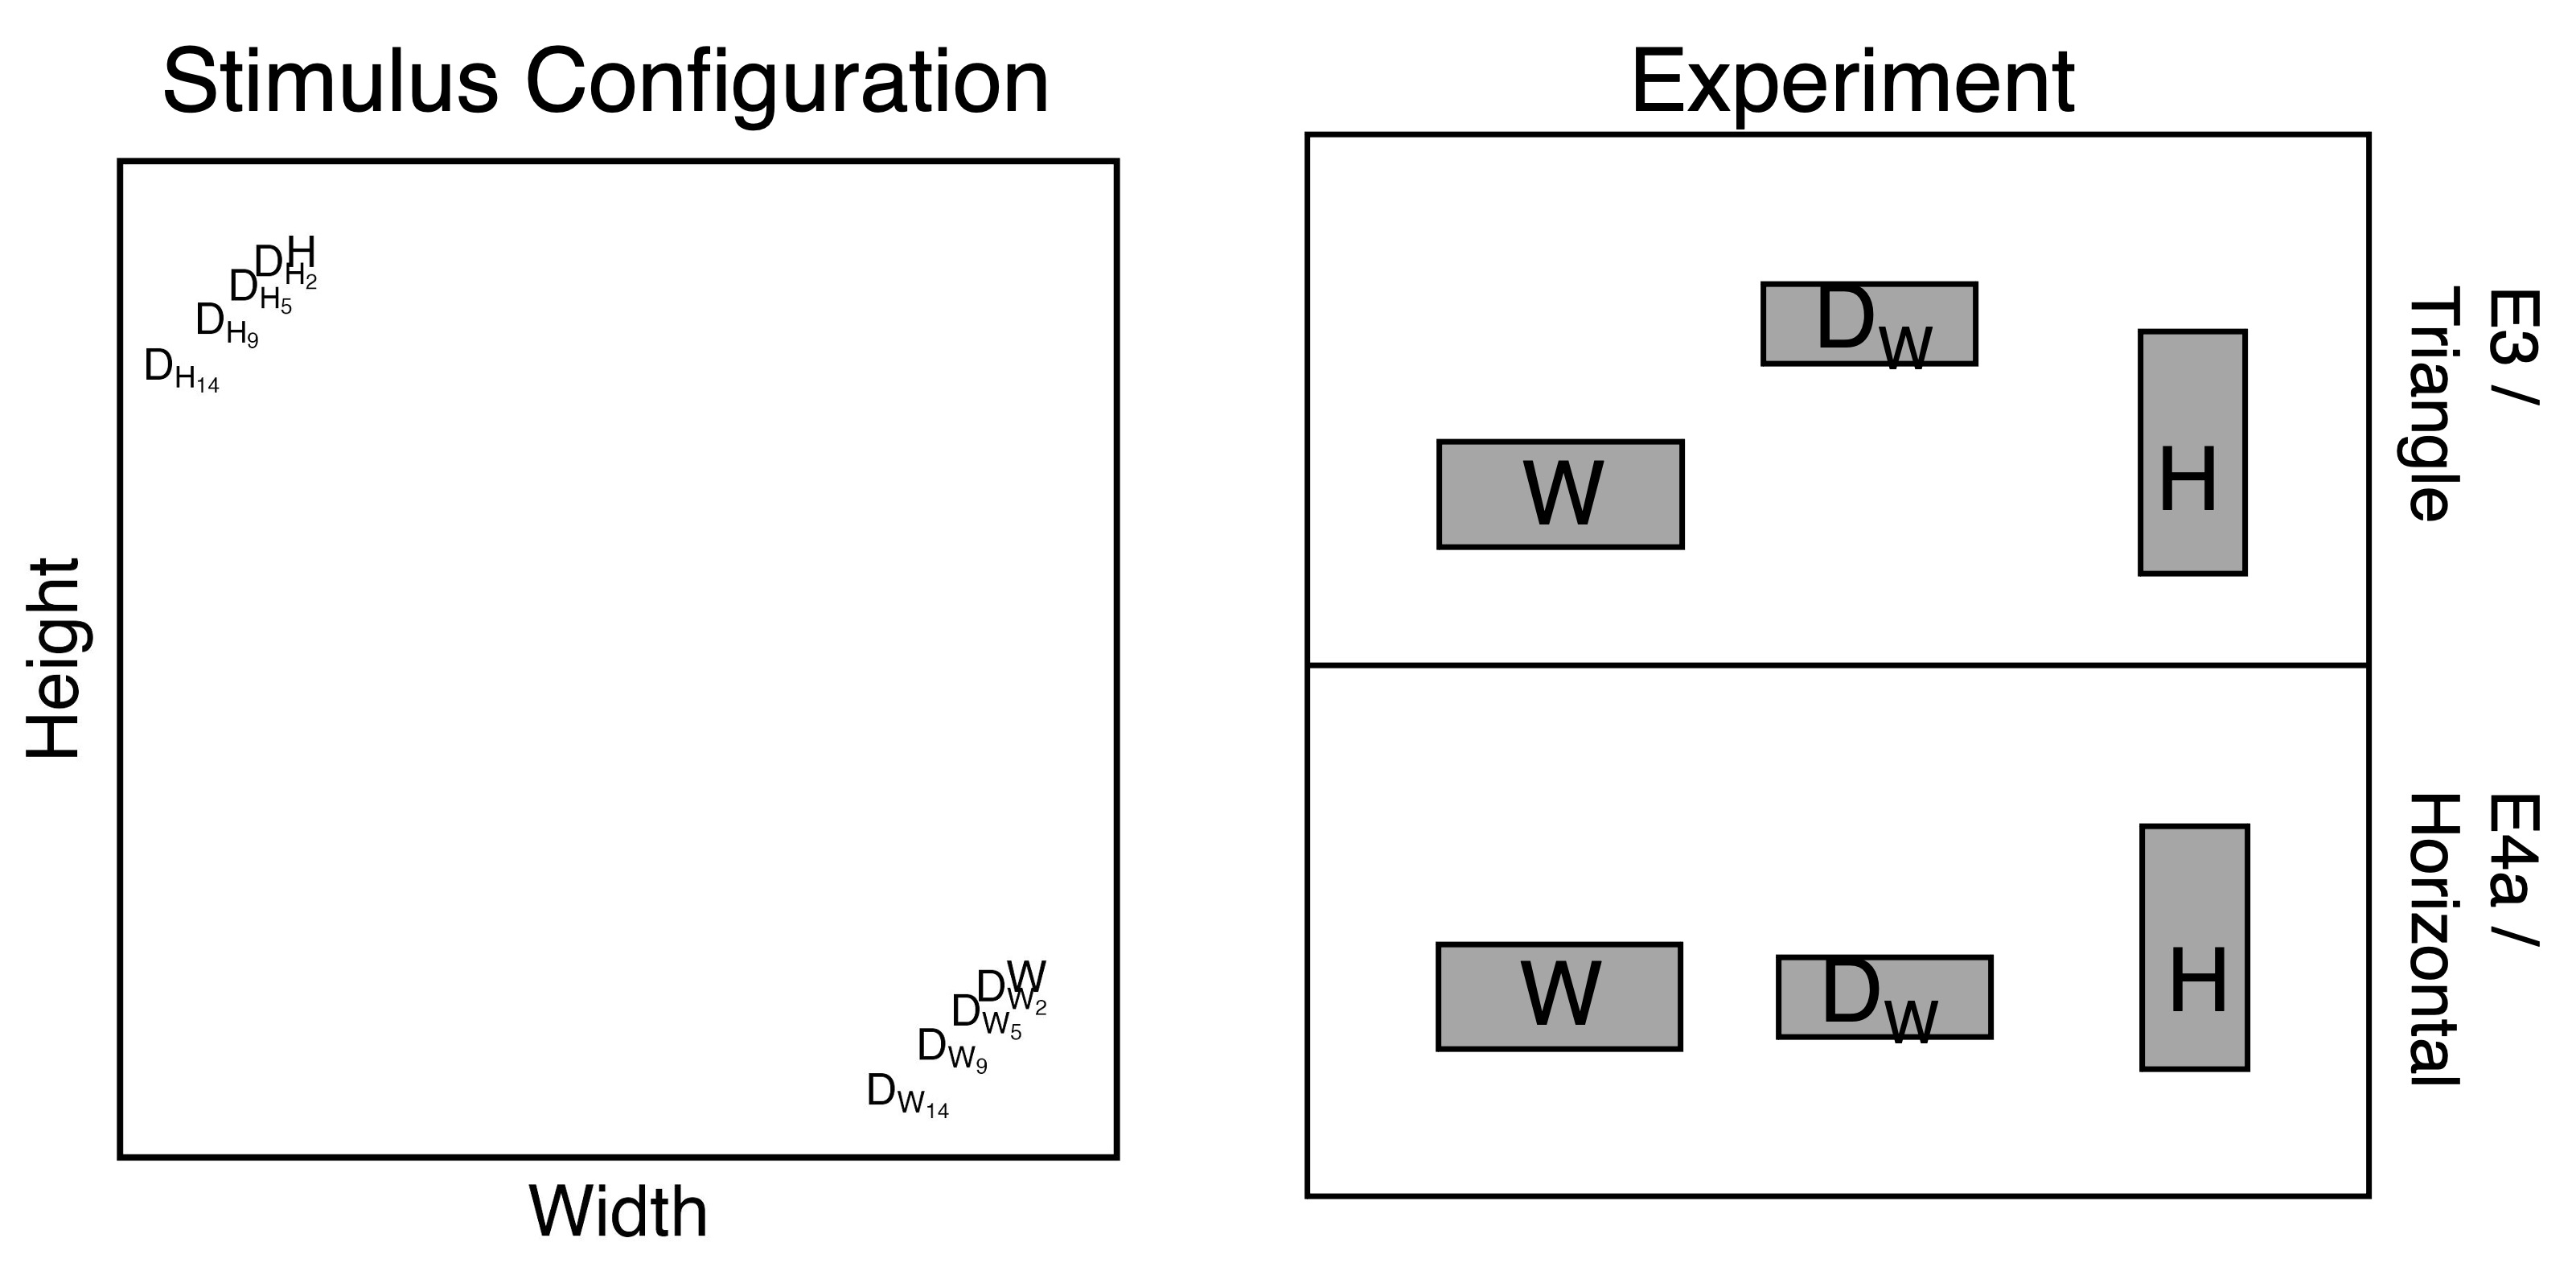
\includegraphics[width=\linewidth]{figures/spektor_stim.png}
   \caption{Stimulus configuration and example trials from \textcite{spektorWhenGoodLooks2018b}, Experiments 3 and 4a.}
   \label{fig:spektor_stim}
\end{figure}

\textcite{spektorWhenGoodLooks2018b} ran a total of five experiments, but I focus on their experiments 3 and 4a here. In Experiment 3, the authors varied TDD at four levels: $2\%$, $5\%$, $9\%$, and $14\%$. The rectangles were arranged in a trianglular display on the screen (see Figure \ref{fig:spektor_stim}, Experiment 3), in contrast to \textcite{trueblood2013not}'s horizontal display. \textcite{spektorWhenGoodLooks2018b} found an empirical repulsion effect such that the competitor was selected more than the target at all levels of TDD (see Figure \ref{fig:spektor_stim}). 

\textcite{spektorWhenGoodLooks2018b} also ran a follow-up experiment using the horizontal diplay of \textcite{trueblood2013not} (see Figure \ref{fig:spektor_stim}, Experiment 4a). Here, they varied TDD at $5\%$, $9\%$, and $14\%$. In Experiment 4a, the data show a slight repulsion effect at low TDD levels that eventually becomes an attraction effect at high TDD levels. 

\begin{figure}
   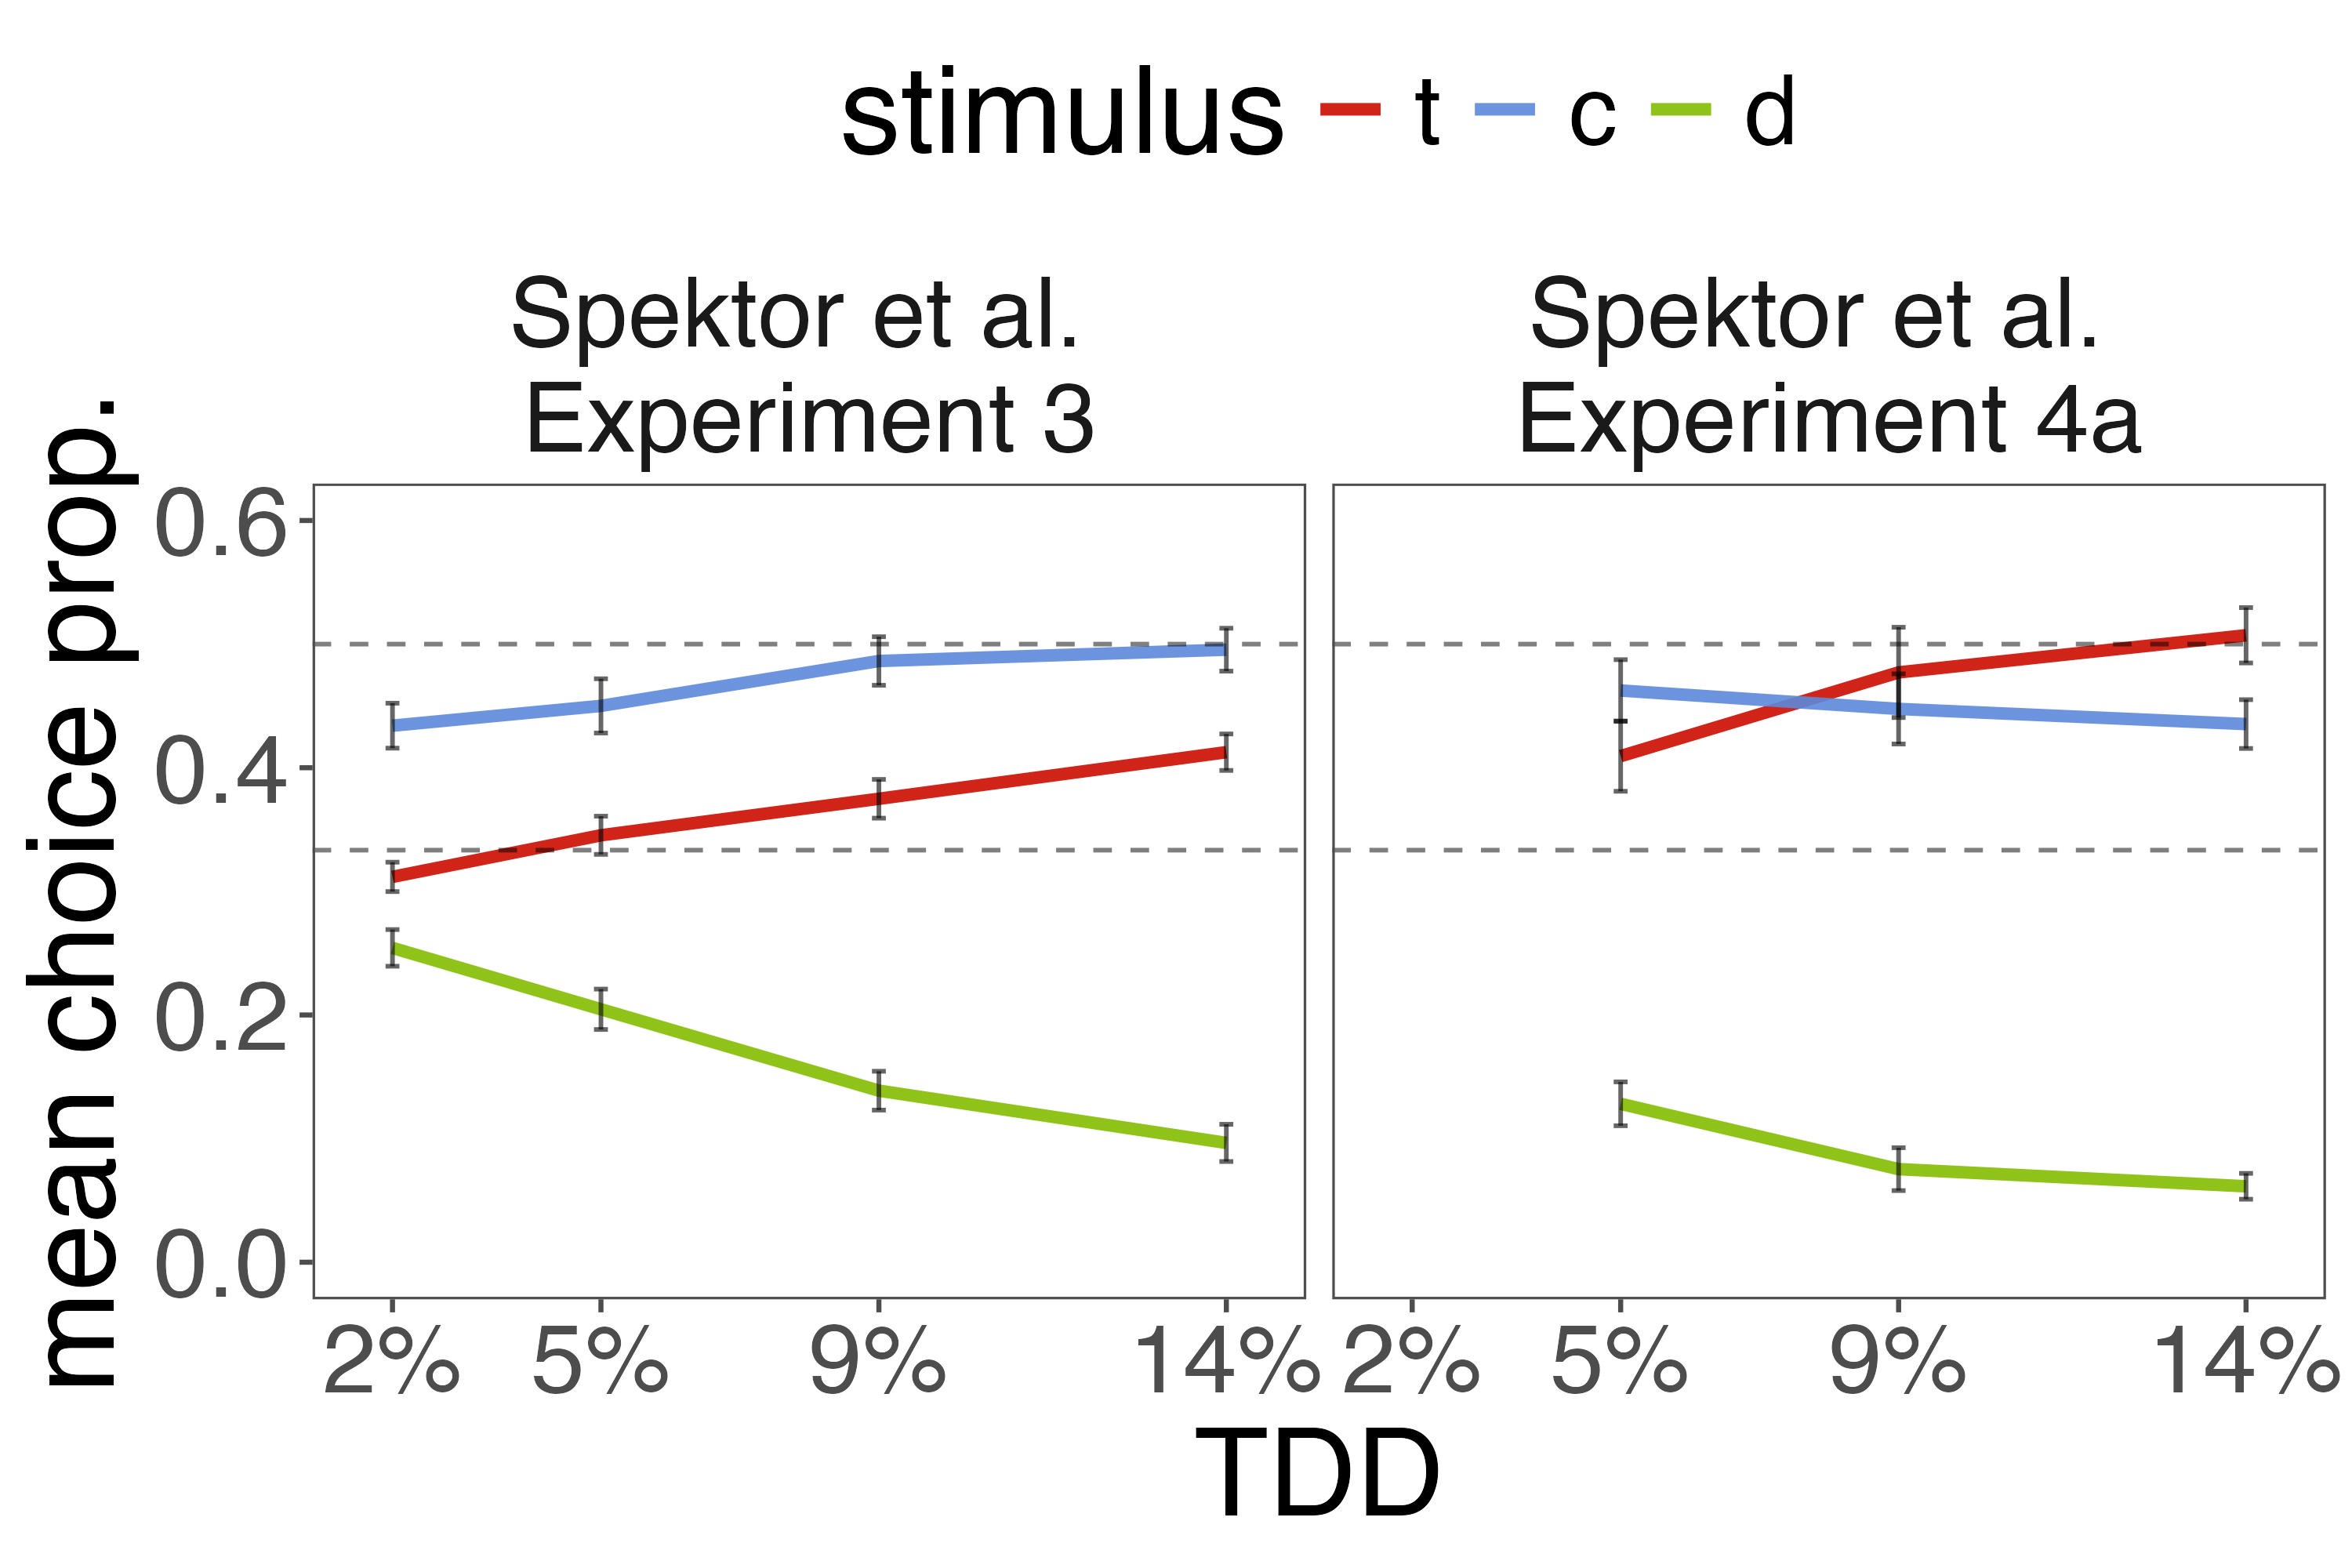
\includegraphics[width=\linewidth]{figures/spektor_data_collapsed.jpeg}
   \caption{Data from \textcite{spektorWhenGoodLooks2018b}, collapsed across choice set. Error bars are $95\%$ CIs of the mean, computed using the within-subjects error correction from \textcite{morey2008confidence}. Dashed lines are drawn at .5 and .33.}
   \label{fig:spektor_data} % might consider graphing (or at least writing RSTs) here
\end{figure}

\textcite{liaoInfluenceDistanceDecoy2021} also replicated the general pattern of \textcite{spektorWhenGoodLooks2018b}'s results and also found a an inverse U-shaped relationship between TDD and RST\footnote{$RST=\frac{P(T|[T,C,D])}{P(T|[T,C,D)+P(C|[T,C,D])}$}. Relatively low and extremely high TDD values created a repulsion effect, while intermediate TDD values created an attraction effect. 

\textcite{spektorRepulsionEffectPreferential2022} demonstrated the repulsion effect in both preferential and perceptual choice, using similar stimuli and display configuration. In these experiments, each stimulus option contained a square with two partially filled bars. In perceptual choice, participants were to select the stimulus with the largest cumulative filled area. In the preferential choice scenario, participants were told that each filled bar represented one possible outcome of a 50-50 gamble, and they were to select the gamble with the highest expected value. Their results were similar to those of \textcite{spektorWhenGoodLooks2018b}, however, where target and competitor choices increased with TDD, with target and decoy showing a particularly strong trade-off.

Researchers are clearly using perceptual experiments to demonstrate context effects and test theory. These results are clearly informative and theoretically interesting. I argue, however, that researchers should be cautious in assuming that decision-makers receive perceptual input with the same accuracy that they do in preferential choice experiments. Researchers should seek to separate the role of perceptual discriminability from decisional processes when understanding participants' responses. I elaborate on these ideas below, with a demonstration using the results of \textcite{spektorWhenGoodLooks2018b}.

\subsection{Understanding Perceptual Choice Experiments}

I seek to understand the role of perception in perceptual choice context effect experiments. To do so, I take an extreme stance - that such experiments are solely perceptual experiments rather than decision-making experiments and that no high level decision processes are occurring. This extreme assumption is incorrect, but I believe it is a good place to start in understanding existing data. I also demonstrate how and under what circumstances it is incorrect later in this dissertation. To begin, I return the results of \textcite{spektorWhenGoodLooks2018b}. 

As reported above, \textcite{spektorWhenGoodLooks2018b} demonstrate that a relatively small change in stimulus display (arranging stimuli in a triangle rather than a horizontal line) reverses the attraction effect. Why is this? To begin to answer this question, I highlight the differences between \textcite{spektorWhenGoodLooks2018b}'s data and previous context effect data. In preferential choice tasks, participants are given a set of options on each trial (e.g., laptops, apartments, washing machines), along with the attribute values associated with each option (e.g., 10 GB RAM, 1500 square feet, 2.7 cubic feet capacity). These attributes are typically represented numerically \parencite{hayes2024attribute,banerjeeFactorsThatPromote2024} or with easily discriminable graphical representations \parencite{cataldoComparisonProcessAccount2019b}. The decoy option, therefore, is rarely selected (e.g., $<5\%$ of all trials), and these selections are assumed to be the result of inattention or accidental responses. Researchers assume that participants are able to detect the dominance relationship between target and decoy. Perceptual choice tasks complicate participants' ability to detect this dominance relationship. In \textcite{spektorWhenGoodLooks2018b}'s experiments, the decoy is selected as often as $25\%$ of all trials in some conditions. The decoy is selected less often in experiment 4a (triangle display) than in experiment 3 (horizontal display). Decoy selections also decrease as the difference between decoy area and target/competitor areas increases. Finally, though both target and competitor increase in choice share as TDD increases, the target choice share increases at a higher rate than does the competitor, suggesting a strong trade-off between target and decoy choices (stronger, indeed, than that of competitor-decoy choices). That is, the mean \textit{Relative Share of the Target} (RST) \parencite{berkowitschRigorouslyTestingMultialternative2014b} increases with TDD in both experiments % should I explicitly show or write mean RST values? -Sean 1/9/25

Clearly, perceptual discriminability plays a role in \textcite{spektorWhenGoodLooks2018b}'s results. Participants clearly are better able to discriminate the target and competitor from the decoy as the decoy decreases in size. Any reasonable account of these data should parse the out discriminability from genuine context effects. 

There is a large body of psychological research, beginning with the work of \textcite{thurstone1927law}, of treating the perception of a stimulus as a random variable. In his famous "Law of Comparative Judgment" paper, \textcite{thurstone1927law} first showed that researchers can use binary choice proportions to estimate the psychological distance between stimuli, by treating perceptual intensity as a Gaussian random variable. This work led to similar research using Signal Detection Theory (STD) \parencite{hautus2021detection}, which also treats psychological quantities (e.g., memory, perception), as random variables. Similarly, Ashby and colleagues' General Recognition Theory (GRT) models the perception of a stimulus as a multivariate normal random variable, where each dimension of the model is the perceived dimension of a stimulus \parencite{ashbyVarietiesPerceptualIndependence1986a,ashby1988decision, ashbyUnifiedTheorySimilarity}. In marketing and economics, researchers treat the utilities of choice options as random variables, which are often assumed to be Gaussian or Extreme Value Distributed and estimate choice models known as Random Utility Models \parencite[RUMs,]{mcfadden2001economic,hausman1978conditional,train2009discrete}.Often, though not necessarily, these models share the common property that value (whether it is the utility of a consumer product, the perception of magnitude, or the memory signal in a recognition task) is stochastic while choice is deterministic \parencite[c.f.,]{benjamin2009signal} I consider this class of models throughout this paper.


\chapter{Parsing Perceptual and Decisional Effects}

\section{Introduction}

I now introduce the model I explore throughout the paper.  This model is simplistic, as it treats the experiments of \textcite{trueblood2013not} and \textcite{spektorWhenGoodLooks2018b} as perceptual, rather than decision tasks. It also completely eschews the possibility of higher level decision processes. I use this model to understand the extent to which. My model treats value (perceived area) as stochastic and choice as deterministic. In my current modeling framework, I do not treat height and width as independent attributes but rather consider perceived area to be unidimensional. In my model, I consider a perceptual choice experiment, where participants are presented with 3 perceptual stimuli on each trial. I asssume that on each trial $i$ with choice set $K$, The perception $\mathbf{X_i}$ of all 3 stimuli is sampled from a multivariate Gaussian distribution with a mean vector $\mathbf{\mu}$ and variance-covariance matrix $\mathbf{\Sigma}$:

\begin{align}
   \mathbf{X_{i}}\sim\mathcal{N}(\mathbf{\mu},\mathbf{\Sigma})
   \label{eqn:mvnorm}
\end{align}

where $\mathbf{\mu}$ is a column vector consisting of:
\begin{align}
   \begin{pmatrix}
      \mu_{T} \\
      \mu_{C} \\
      \mu_{D}
      \end{pmatrix}
   \label{eqn:mu}
\end{align}

where the subscripts $T$, $C$, and $D$ indicate target, decoy, and competitor, respectively, and $\mathbf{\Sigma}$ is a positive semi-definite 3x3 covariance matrix computed as:

\begin{align}
   \mathbf{\Sigma}=S\mathbf{\Omega}S
   \label{eqn:Sigma}
\end{align}

where $S$ is a diagonal matrix consisting of: 

\begin{align}
   \begin{pmatrix}
      \sigma_{T} & 0 & 0 \\
      0 & \sigma_{C} & 0 \\
      0 & 0 & \sigma_{D} \\
   \end{pmatrix}
   \label{eqn:R}
\end{align}

and $\Omega$ is a correlation matrix:

\begin{align}
   \begin{pmatrix}
      1 & \rho_{TC} & \rho_{TD} \\
      \rho_{TC} & 1 & \rho_{CD} \\
      \rho_{TD} & \rho_{CD} & 1 \\
   \end{pmatrix}
   \label{eqn:R}
\end{align}

with $\rho_{TD}$, for example, indicating the population-level correlation between target and decoy stimuli.

As mentioned above, the model assumes that value is stochastic while choice is deterministic\footnote{This also assumes ties are not possible, which is true if and only if perceived area is absolutely continuous.}. The model always "selects" the option perceived the largest, regardless of the magnitude of the difference between the "winner" and "runners-up". That is, given a vector $X_{i}$ of perceived areas on trial $i$ with set $K$, the probability a participant selects stimulus $i$ is:

\begin{align}
   P(i|K)=P(X_{i}>X_{j}, j \in K, i \neq j)
   \label{eqn:pchoice}
\end{align}

When any elements of $\Omega$ are non-zero, the closed form solution of this model does not exist, and to compute predictions, researchers must use simulation or numerical integration methods \parencite{train2009discrete}. In all applications of these model through this dissertation, I use simulation to generate model predictions.

I consider the role of perceptual correlations between all pairs of stimuli, i.e., $\rho_{TC}$, $\rho_{TD}$, and $\rho_{CD}$. I vary both $\rho_{TD}$ and $\rho_{TC}$ from -1 to 1; in other words, all rectangles oriented the same way share one correlation and those oriented differently share another correlation. I show model predictions that result from varying these correlations in Figure \ref{fig:3d_model}. Here, I assume that $\mu_{T}=\mu_{C}>\mu_{D}$ and that $\sigma_{T}=\sigma_{C}=\sigma_{D}$\footnote{In Experiment 2 I present evidence supporting the former assumption. I also relax the latter assumption when modeling Experiment 2}. 

\ref{fig:3d_model} shows model predictions in the form of $RST$ (Relative Share of the Target), where RST values above .5 indicate an attraction effect and values below .5 indicate a repulsion effect. My model can, depending on the relationship between $\rho_{TD}$ and $\rho_{TC}$, predict a repulsion, attraction, or a null context effect. If $\rho_{TD}>\rho_{TC}$, the model predicts a repulsion effect. If the target and decoy are correlated more strongly than competitor and decoy, it is more likely that if on a particular trial the target perception is large, that the decoy is even \textit{larger}, causing the decoy to "steal" choice shares from the target more than the competitor, i.e., a repulsion effect.

If $\rho_{TD}<\rho_{TC}$, the model predicts an attraction effect. This is because $\rho_{TC}=\rho_{CD}>\rho_{TD}$, so the decoy "steals" choice shares from the competitor more than the target. 

Finally, if $\rho_{TD}=\rho_{TC}=\rho_{CD}$, the model predicts a null effect. In this case, no pair of stimuli are more correlated than any other pair, so the predictions are identical to a model where $\rho_{TD}=\rho_{TC}=\rho_{CD}=0$ model. This model collapses to an Independent Normal Model. 

\begin{figure}
   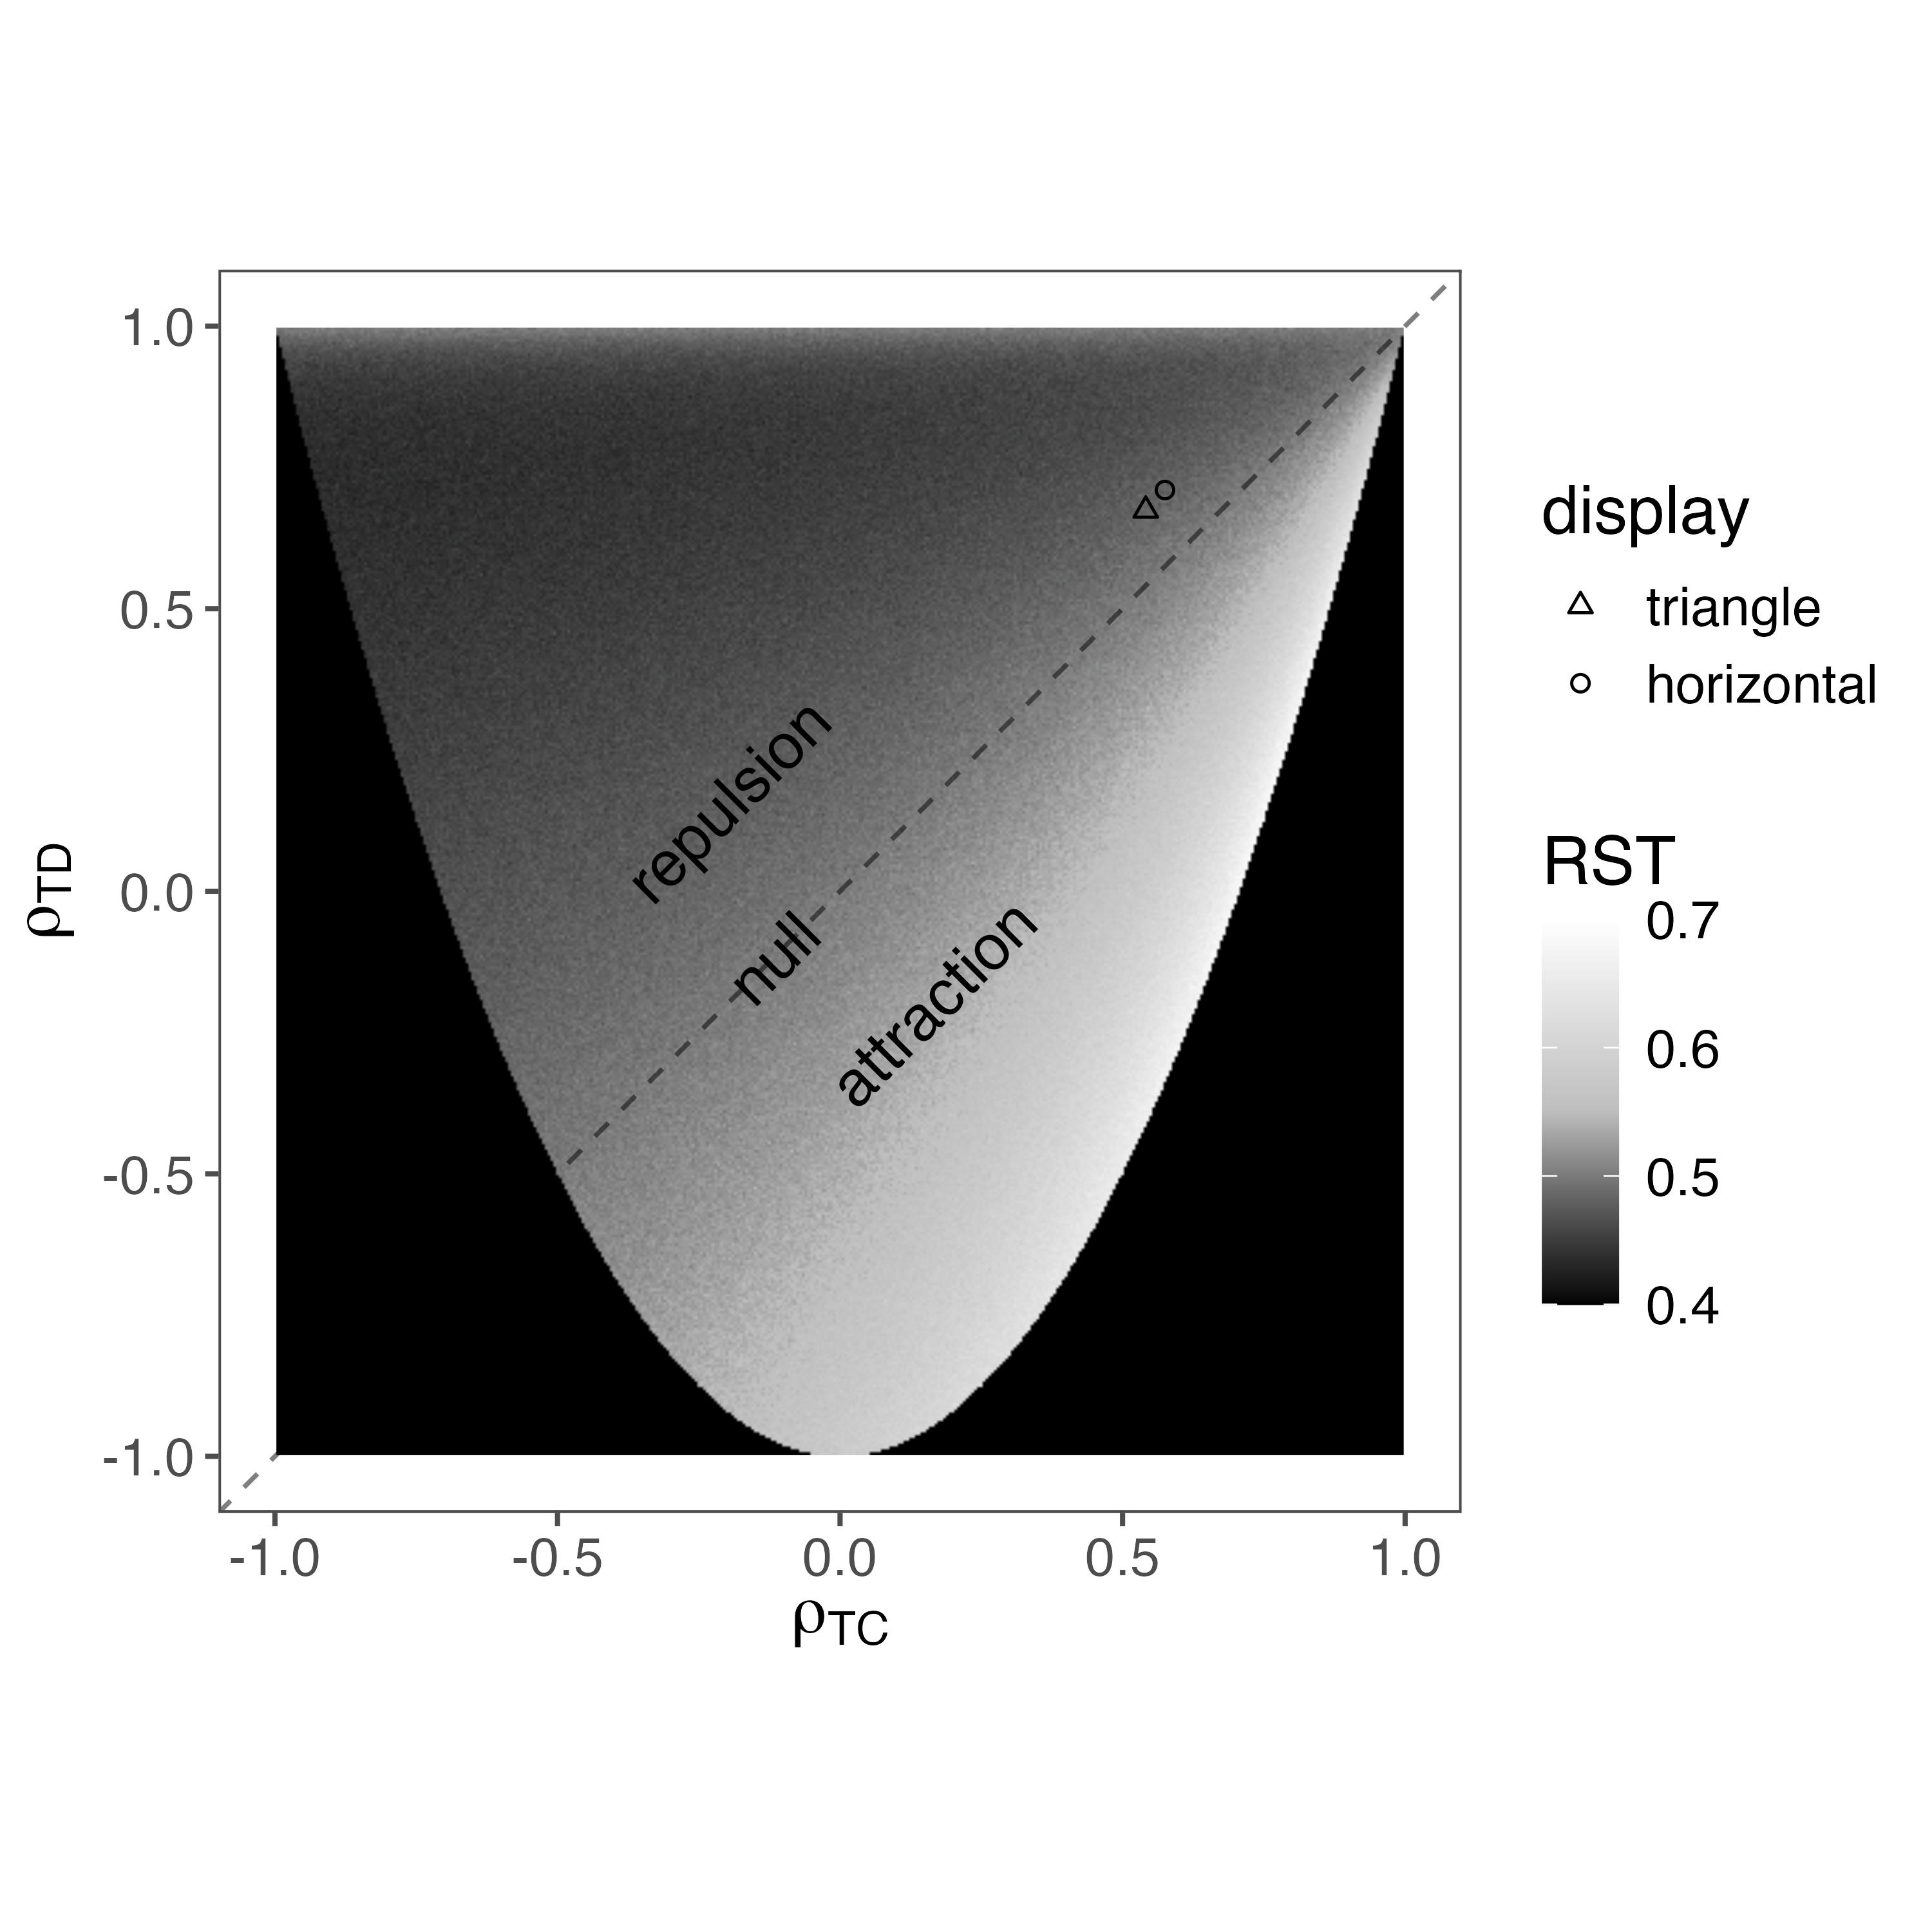
\includegraphics[width=\linewidth]{figures/3d_sim_rst.jpg}
   \caption{Model simulations for the attraction and repulsion effects based on the variation of $\rho_{TD}$ and $\rho_{TC}$. "Regions" of the plot are labeled based on their qualitative predictions for attraction, null, and repulsion effects. The black region is the area where, due to extreme correlations, a positive semi-definite variance-covariance matrix could not be formed and predictions are unavailable. The triangle and circle mark the observed mean correlations from the Experiment 2 triangle and horizontal conditions respectively.}
   \label{fig:3d_model}
\end{figure}

\subsection{Accounting for perception}
I propose that these perceptual correlations may be driving the repulsion effect in \textcite{spektorWhenGoodLooks2018b}'s data. The decoy option is smaller than the the target and competitor options and is thus not always discriminated. The triangle configuration makes discriminability particularly difficult for participants (as I show below in my Experiment 1). Simultaneously, however, the fact that target and decoy share an orientation (i.e., both wide or both tall) makes the comparison of these two options easier. In statistical terms, the perception of the decoy is more strongly correlated with the perception of the target than with perception of the competitor. Given these correlations, the perceived area of the decoy is more likely to exceed the target than the competitor. Conceptually, an empirical repulsion effect may be driven by perception rather than the "high-level" effects typically considered in the decision-making literature.

Modern psychological models of context effects often assume an attribute-wise comparison process \parencite{roeMultialternativeDecisionField2001a,trueblood2013not,usherLossAversionInhibition2004a,bhatiaAssociationsAccumulationPreference2013b}. Under this class of models, participants arrive at a decision by comparing pairs of options on a single attribute, where the modeller assumes attribute values are veridical. This assumption is quite reasonable when modeling choices where each attribute is presented separately and discriminability issues are minimal or non-existent. In this article, I present evidence that this assumption may not be appropriate. ELABORATE HERE

In Experiment 1, I first present results from a two-alternative forced-choice experiment to show that these stimuli are easily confusable and that the triangle display of \textcite{spektorWhenGoodLooks2018b} decreases discriminability relative to the triangle display. I also show that, consistent with the predictions of a perceptual model where $\rho_{TD}>\rho_{TC}>\rho_{CD}$, target-decoy discriminability is in fact \textit{easier} than competitor-decoy discriminability and that target-decoy discriminability increases with TDD. 

In Experiment 2, I combined a psychophysics task with a choice task to estimate the parameters of my perceptual model. In the first phase of the experiment, participants estimate the size of target, decoy, and competitor rectangles on each trial. In the second phase of the experiment, I conducted a standard choice experiment, replicating \textcite{spektorWhenGoodLooks2018b}'s results. I use the data from the first phase of Experiment 2 to obtain stable estimates of  $\mathbf{\mu}$ and $\mathbf{\Sigma}$ in my perceptual model. Finally, I show that the model, conditioned on the observed parameter estimates, naturally predicts a repulsion effect but not an attraction effect.  

\section{Experiment 1}

The goal of Experiment 1 was to test participants' ability to discriminate between rectangles in the perceptual choice tasks of \textcite{trueblood2013not} and \textcite{spektorWhenGoodLooks2018b}. I do, however, acknowledge the possibility that the presentation of three options (rather than just two) may impact perception. 
On each trial, I presented participants with three options (target, competitor, and decoy). After a short delay, I highlighted two of the three rectangles and asked participants to indicate which rectangle was larger. 
Additionally, I used a within-subjects manipulation to compare discriminability in both the triangle display of \textcite{spektorWhenGoodLooks2018b}, Experiment 3, and the horizontal display of \textcite{spektorWhenGoodLooks2018b}, Experiment 4a\footnote{see also \textcite{trueblood2013not}, Experiment 1.}. Otherwise, with a few exceptions discussed below, I follow the stimulus construction and experimental design of \textcite{spektorWhenGoodLooks2018b}, Experiment 3. 

\subsection{Methods}

\subsubsection{Participants.}
Data collection took place at the University of Massachusetts Amherst. 86 undergraduate students participated in exchange for course credit. 1 participant who achieved less than $80\%$ accuracy on catch trials (see below) was excluded from all analyses. Trials with response times (RTs) $<100\text{ms}$ or  $>10000\text{ms}$ were also excluded from all analyses.

\subsubsection{Stimuli.}
The experiment had two types of trials: critical trials and catch trials. 
On each critical trial, the target and competitor had the same area\footnote{Here I simplify \textcite{spektorWhenGoodLooks2018b}'s design by ensuring both focal stimuli had the same area.} but differed on orientation, with one stimulus being wide and the other tall. The decoy always had the same orientation as the target. The height and width of the decoy were reduced proportionally so that the decoy area was always $0\%$, $2\%$, $5\%$, $9\%$, or $14\%$ of the target areas. Because the target and competitor always had the same area, this means that the decoy was also $0\%$, $2\%$, $5\%$, $9\%$, or $14\%$ of the competitor area. These are the TDD values from \textcite{spektorWhenGoodLooks2018b}, plus a $0\%$ level which acted as a baseline\footnote{When TDD=$0\%$, the target and decoy are identical, so labeling is arbitrary.}.

\subsubsection{Design.}
There were 5 blocks of trials. In each block there were 60 critical trials, 12 at each TDD level, and 30 catch trials. Of the 12 critical trials at each TDD level, 6 were presented in a triangle and 6 were presented horizontally. Finally, 3 of the 6 targets in each display condition at each TDD level were wide and 3 were tall. Of each of these 3, one was a target-decoy comparison, one was a target-competitor comparison, and one was a target-competitor comparison. Trial order and rectangle order within each trial were randomized.

On each catch trial, there was one large rectangle and two much smaller rectangles. The large rectangle was $260 \pm U(-40, 40) \text{x} 200 \pm U(-40, 40)$ pixels, with a random orientation. The smaller rectangles were $180 \pm U(-40, 40) \text{x} 120 \pm U(-40, 40)$ pixels, one wide and one tall.

On every trial, the rectangles were displayed in either a triangle or horizontal display (see \ref{fig:spektor_stim}). The horizontal distance between all rectangles was constant, but 25 pixels of jitter was added to each rectangle's vertical location.

Stimuli were presented on computer monitors with a resolution of 1920 x 1080 pixels. The experiment was programmed with jsPsych \parencite{deleeuwJsPsychJavaScriptLibrary2015}. 

\subsubsection{Procedure.}
On each trial, participants saw three rectangles, labeled 1, 2, and 3 (from left to right). The rectangles appeared for 1825ms total, but after 500ms, two of the rectangles changed to a darker shade. After all three rectangles disappeared from the screen, participants were asked to select which of the two darker rectangles had the larger area.

\subsection{Results}

\subsubsection{Catch Trials.}
Participants performed well on the catch trials. The mean percentage correct in the triangle display was $92.6\% (SD=3.77)$, and the mean percentage correct in the triangle display was $93.2\% (SD=3.52)$. 

\subsubsection{Critical Trials.}
I first checked the baseline TDD level data (TDD=$0\%$) across to make sure that participants were indifferent between pairs of options when they had identical area. The mean percentage of target choices in target-competitor trials was $48.99\%$ (SD=10.18). The mean percentage of competitor choices in competitor-decoy trials was $49.80\%$ (SD=11.30). The mean percentage of target choices in target-decoy trials was $49.47\%$ (SD=12.06). Participants were indifferent between all pairs of options in the $\text{TDD}=0\%$ trials, so I do not consider these trials further.

The primary analysis was performed on the target-decoy and competitor-decoy trials, excluding the TDD=$0\%$ trials. In these trials participants' task is simply to not select the decoy option on a given trial. I present mean choice proportions across conditions in Figure \ref{fig:e1_data}. Participants' performance indeed improves with TDD. Furthermore, their performance is better when stimuli are displayed in the horizontal configuration than in the triangle configuration, and it is also better in target-decoy trials compared to competitor-decoy trials. Finally, there is an interaction, such that as TDD increases, the target-decoy performance is even better than the competitor-decoy performance. See Appendix XXX for inferential statistics which support these conclusions.

\begin{figure}
   \includegraphics[width=\textwidth]{figures/m6_model_preds_v_data.jpeg}
   \caption{Experiment 1, mean choice proportions by stimulus display, TDD, and comparison. td=target-decoy trials, dc=competitor-decoy trials. Model predictions come from the Bayesian hierarchical logistic regression presented in Appendix XXX. Error bars are $95\%$ HDIs on the mean.}
   \label{fig:e1_data}
\end{figure}

\subsubsection{Discussion}
In Experiment 1, I showed that participants are not always able to discriminate between target-decoy and competitor-decoy stimuli. I also show that this discriminability increases with TDD and that overall discriminability is better in the horizontal compared to the triangle display. Finally, through the interaction of comparison-pair and TDD, I show that target-decoy discriminability increases with TDD at a higher rate than competitor-decoy discriminability. 

These results, in fact, are natually predicted by a model where $\rho_{TD}>\rho_{CD}$ (see Appendix XXX for simulations - NEED TO DO THIS).

\subsection{Experiment 2}
I continue this line of research in Experiment 2, where I used a psychophysics task to estimate the mean perceived area and correlations between perceived area to the target, competitor, and decoy rectangles. Experiment 2 used the \textit{method of cross-modal matching} \parencite{stevensCrossmodalityMatchingBrightness1965}, where participants adjusted the size of a circle to match the perceived area for each rectangle. On each trial, participants saw three rectangles and three circles, each labeled 1, 2, and 3. Participants adjusted the size of the circle corresponding to each rectangle, until they believed the two to have equal area. I also replicate \textcite{spektorWhenGoodLooks2018b}'s choice data in a second phase of the experiment. Finally, I used a between-subjects manipulation to display the rectangle stimuli in either the horizontal or triangle displays of \textcite{spektorWhenGoodLooks2018b}.

\subsubsection{Methods}
\subsubsubsection{Participants.}
Data collection took place at the University of Massachusetts Amherst. 521 undergraduate students participated in exchange for course credit. 68 participants did not complete the full experiment within the 1 hour time limit and were removed from all analyses. 

\subsubsubsection{Stimuli.}
In the circle adjustment phase there were three types of trials: critical trials, filler trials, and catch trials. On each critical trial, the target and competitor had the same area but differed on orientation, with one stimulus being wide and the other tall. The decoy always had the same orientation as the target. I varied TDD at $2\%$, $5\%$, $9\%$, and $14\%$. I also varied the target, competitor, and decoy stimuli to fall on three diagonals. In pixels, the small and larger focal stimulus dimension values on the lower, middle, and upper diagonals were $[60, 135]$, $[90, 165]$, and $[120,195]$. I reduced the absolute size of the target/competitor stimuli from Experiment 1 to Experiment 2 to accomodate the circle adjustment phase (see procedure  below).

On filler trials, I randomly sampled three rectangles by sampling a height and width from the distribution $U(56,195)$, encompassing the full range of stimuli from the critical trials.

On the catch trials, I randomly sampled one rectangle from the lower diagonal and two from the upper diagonal, so one stimulus was clearly larger than the other two.

The choice phase had identical trial types with the exception that there were no catch trials, only critical and filler trials.

\subsubsubsection{Design.}
Across both phases, I varied display condition between-subjects and TDD, diagonal, target-decoy orientation within-subjects. After removing subjects, there were 218 participants in the horizontal display condition and 225 participants in the triangle display condition. 

In the circle adjustment phase, there were 4 blocks, each 40 trials. Each block consisted of 24 critical trials, 14 filler trials, and 2 catch trials. Within the critical trials, there were 6 trials at each level of TDD. In 3 of these 6 trials the target and decoy were oriented wide (choice set $[w,h,d_{w}]$), and in the other 3 target and decoy were oriented tall (choice set $[w,h,d_{h}]$). 

In the choice phase, there were 4 blocks, each with 34 trials. 24 of these trials were critical trials and 10 were filler trials. Of these 24 critical trials, there were 6 trials at each level of TDD. Within each 6, there were 3 trials where target and decoy were oriented wide and 3 were target and decoy were oriented tall. 

\subsubsubsection{Procedure.}

The experiment took place in two phases: 

On each circle adjustment trial, three gray rectangles appeared in the lower left corner of the screen, either in a triangle or horizontal display. In the upper right, three gray circles appeared in the upper right of the screen, in the same display as the rectangles (see Figure \ref{fig:circle_exp_display} ). A small amount of jitter ($U(-15,15)\text{px}$) was added to the position of each rectangle and the corresponding circle. Each circle started with an area of 78 square pixels (i.e., with a radius of 5), the minimum size I allowed in the experiment. Participants used the mouse to adjust the circle. Within a single trial, they were free to adjust the circles in any order they liked or to go re-adjust a circle as much as they liked. There was no time limit to each adjustment trial. The maximum circle area allowed was 65144 square pixels\footnote{I arrive at this number based on the maximum area the circles could be while only appearing on the right half of the screen and maintaining the same horizontal distance from each other as the corresponding rectangles.}. When a participant finished adjusting the circles on a trial, they clicked the "Submit" button located on the lower right hand corner of the screen. 

The circle adjustment phase began with three practice trials, followed by the 4 blocks of experimental trials. At the beginning of each experimental block, participants completed 3 calibration trials. Calibration trials were identical to filler trials, with the caveat that I provided feedback after participants' responses. After participants submitted their responses on a trial, a red circle appeared around each adjusted circle, showing the true area of the corresponding rectangle. 

Throughout the circle phase, I kept track of the deviations between the true rectangle areas and the participants' adjusted circle areas. At the end of each block, I computed the current mean deviation, and, depending on this value, told the participant that they were either over or under-adjusting, on average.

The choice phase began with 3 practice trials. Participants were not provided feedback during these practice trials. 

On each choice trial, three rectangles appeared in the center of the screen in a horizontal or triangle display. There was no vertical jitter added here. Participants were told to select the rectangle with the largest area by clicking on it.

At the end of the choice phase, I let each participant know their percentage correct from the choice phase. Note that in a critical trial, a correct response is simply one where they did not select the decoy, as the target and competitor rectangles always had the same area.

Stimuli were presented on computer monitors with a resolution of 1920 x 1080 pixels. The experiment was programmed with GNU Octave \parencite{octave} and PsychoPhysics Toolbox \parencite{brainardPsychophysicsToolbox1997}. 

\begin{figure}
   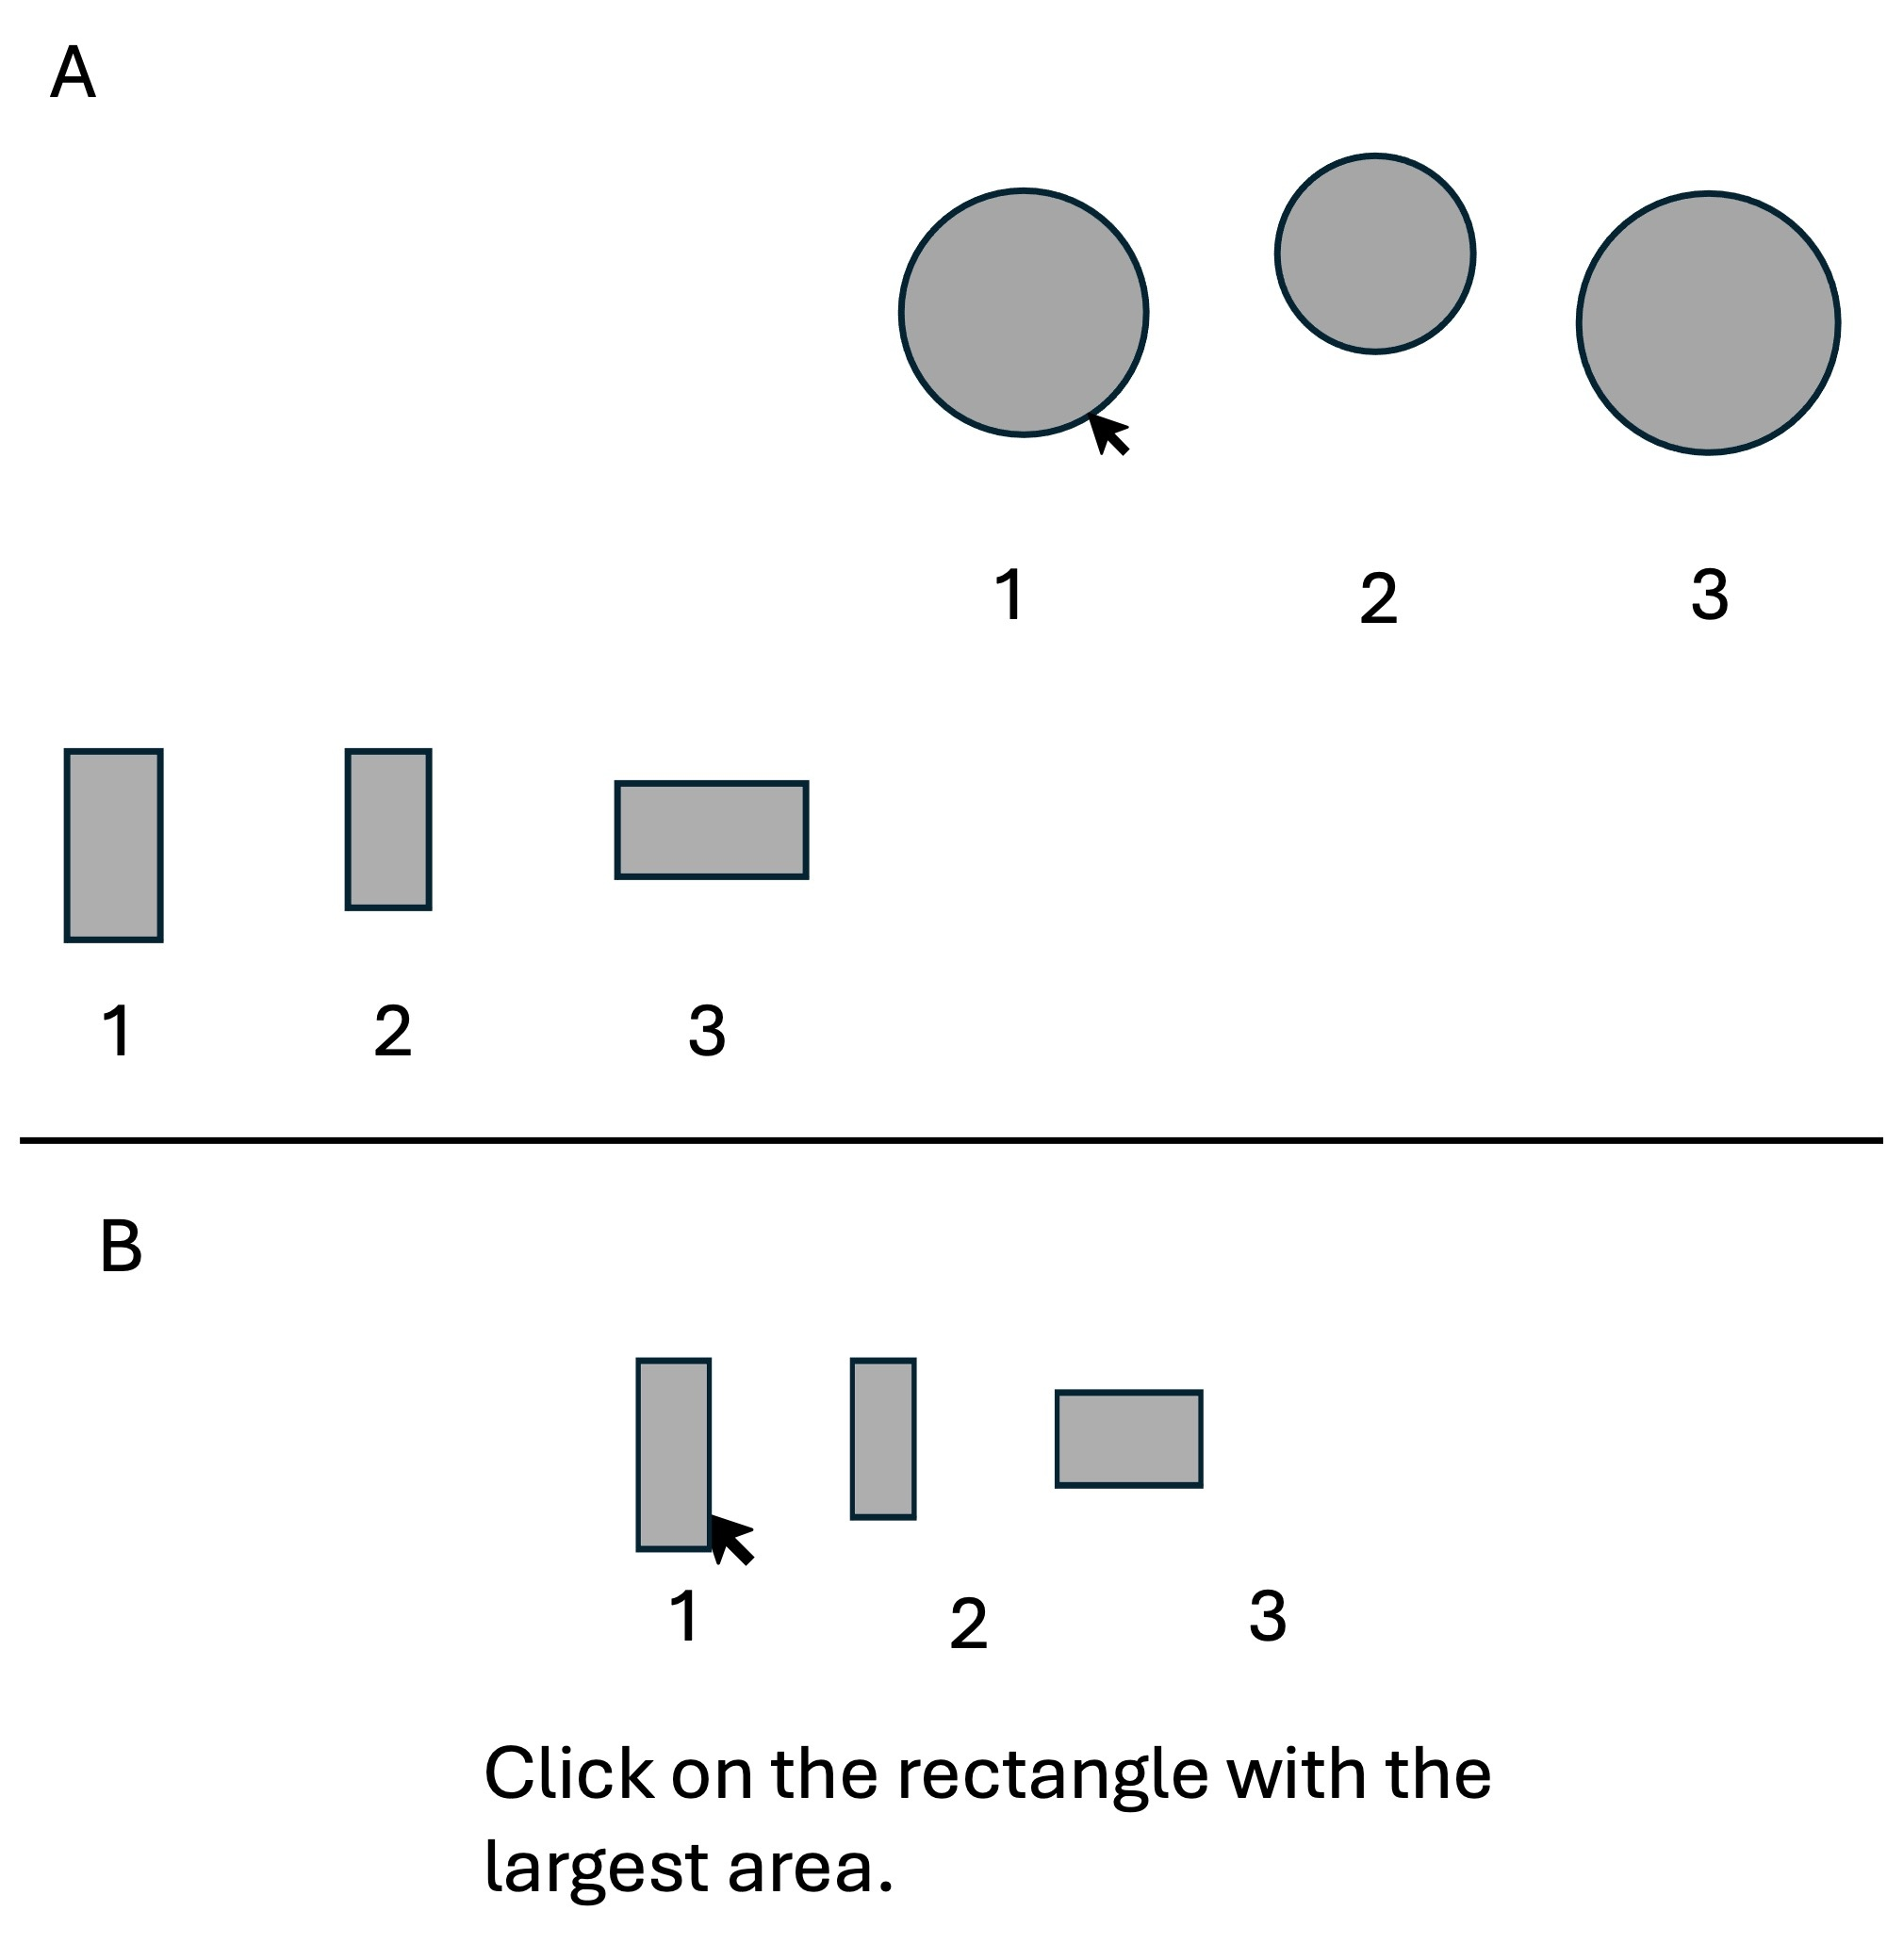
\includegraphics[width=\linewidth]{figures/circle_exp_display.jpg}
   \caption{Example trials from Experiment 2. A: Circle adjustment phase. B: Choice phase. This an example of trials in the horizontal display condition.}
   \label{fig:circle_exp_display}
\end{figure}

\subsubsection{Results}
\subsubsubsection{Data Processing}
Given the difficulty of the circle adjustment task, the data required processing to ensure that outlier trials and participants did not influence our estimates of $\mathbf{Omega}$.

First, I removed all participants who did not give correct responses on $75\%$ ($6/8)$ of the catch trials. A correct response entails estimating the larger rectangle to be the largest on the trial. 10 participants were removed from all analyses after they failed to achieve at least $75\%$ correct on catch trials (see below for details). This left a total of 443 participants.

Next, from the remaining participants, I first natural log-transformed all responses. I then dropped all trials where at least one circle was not adjusted (i.e., at least one circle was left at the starting size).

I then removed outlier participants using the following procedure:

I fit a linear regression to each individual participants' data, regressing each log circle area on each corresponding log rectangle area. I then computed an $R^2$ for each participant. I then removed all participants whose $R^2$ fell below the $5\%$ quantile for all $R^2$s, which in this case was $.3975$. This removed 23 subjects, leaving us with a total of 420 participants, 213 in the triangle display condition and 207 in the horizontal display condition. Of the remaining participants, $R^2$ values were high ($M=.67,SD=.12$), indicating they could generally perform the task.

From the $420$ partipants whose data I analyzed, I removed outlier trials from the critical trial data. I did so to ensure that any outliers do not influence our estimates of $\rho_{TD}$, $\rho_{TC}$, or $\rho_{CD}$. I z-transformed all log circle areas within each participant and diagonal. I remove all critical trials where at least one z-score had an absolute value above $3.5$. This led to $102$ trials being dropped. I dropped $0$, $1$, $2$, and $4$ critical trials from $339$, $62$, $18$, and $1$ participants, respectively. 

After all circle phase data processing, I were left with $20371$ trials in the triangle display condition and $19809$ trials in the horizontal display condition. 

For the choice phase, I only retained participants whose data I retained in the circle phase.

\subsubsubsection{Circle Phase Results - Critical Trials}
Before modeling our data, I wanted to ensure that participants could successfully perform the task. While I do not expect perfect performance in an absolute sense, I do require adequate relative performance. 

To assess performance on the critical trials, I computed the mean difference between actual log area and estimated log area for each subject, stimulus pair (i.e., target-competitor, target-decoy, competitor-decoy), and actual difference. I plot these via a set of boxplots in Figure \ref{fig:circle_boxplots}. Although participants vary considerably in their judgments, I find that on average, participants' adjusted circle areas increase with the absolute size of rectangles. 


\begin{figure}
   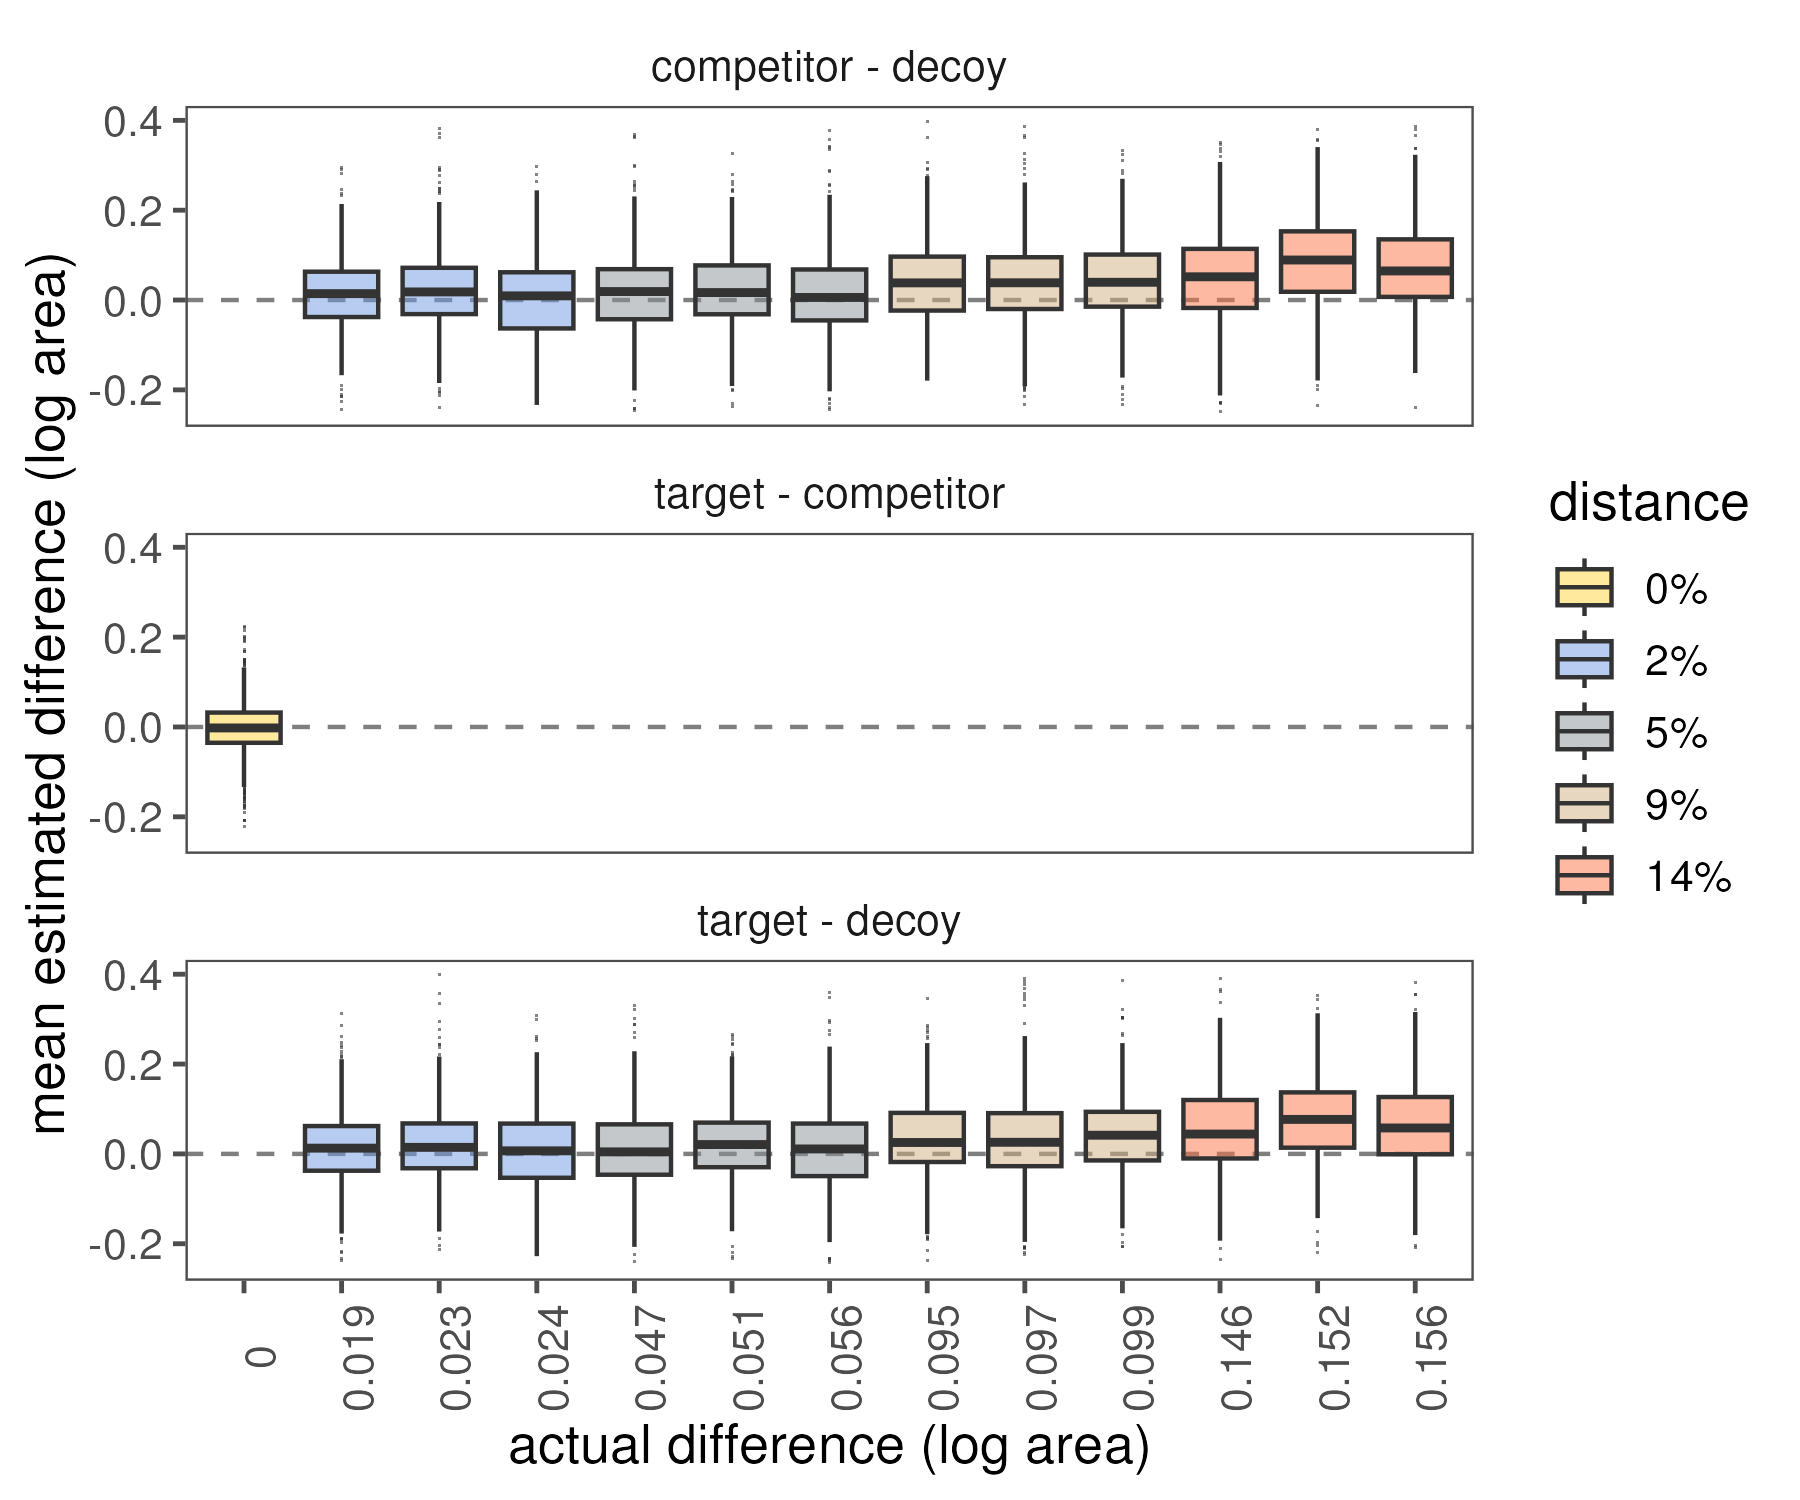
\includegraphics[width=\textwidth]{figures/circleAreaPhase_boxplot_meanlogdiffs_no_outliers.jpeg}
   \caption{Boxplot of subject-level mean error in area estimations, split by stimulus pair, TDD, and absolute discrepancy in rectangle area. Note that because the target and competitor rectangles always had equal areas, the true difference is always 0.}
   \label{fig:circle_boxplots}
\end{figure}

I next present scatterplots of all pairwise circle areas from each trial, see Figure \ref{fig:raw_cors}. I present these to be transparent about the raw data and to illustrate the necessity of a statistical model to understand these correlations. 

\begin{figure}
   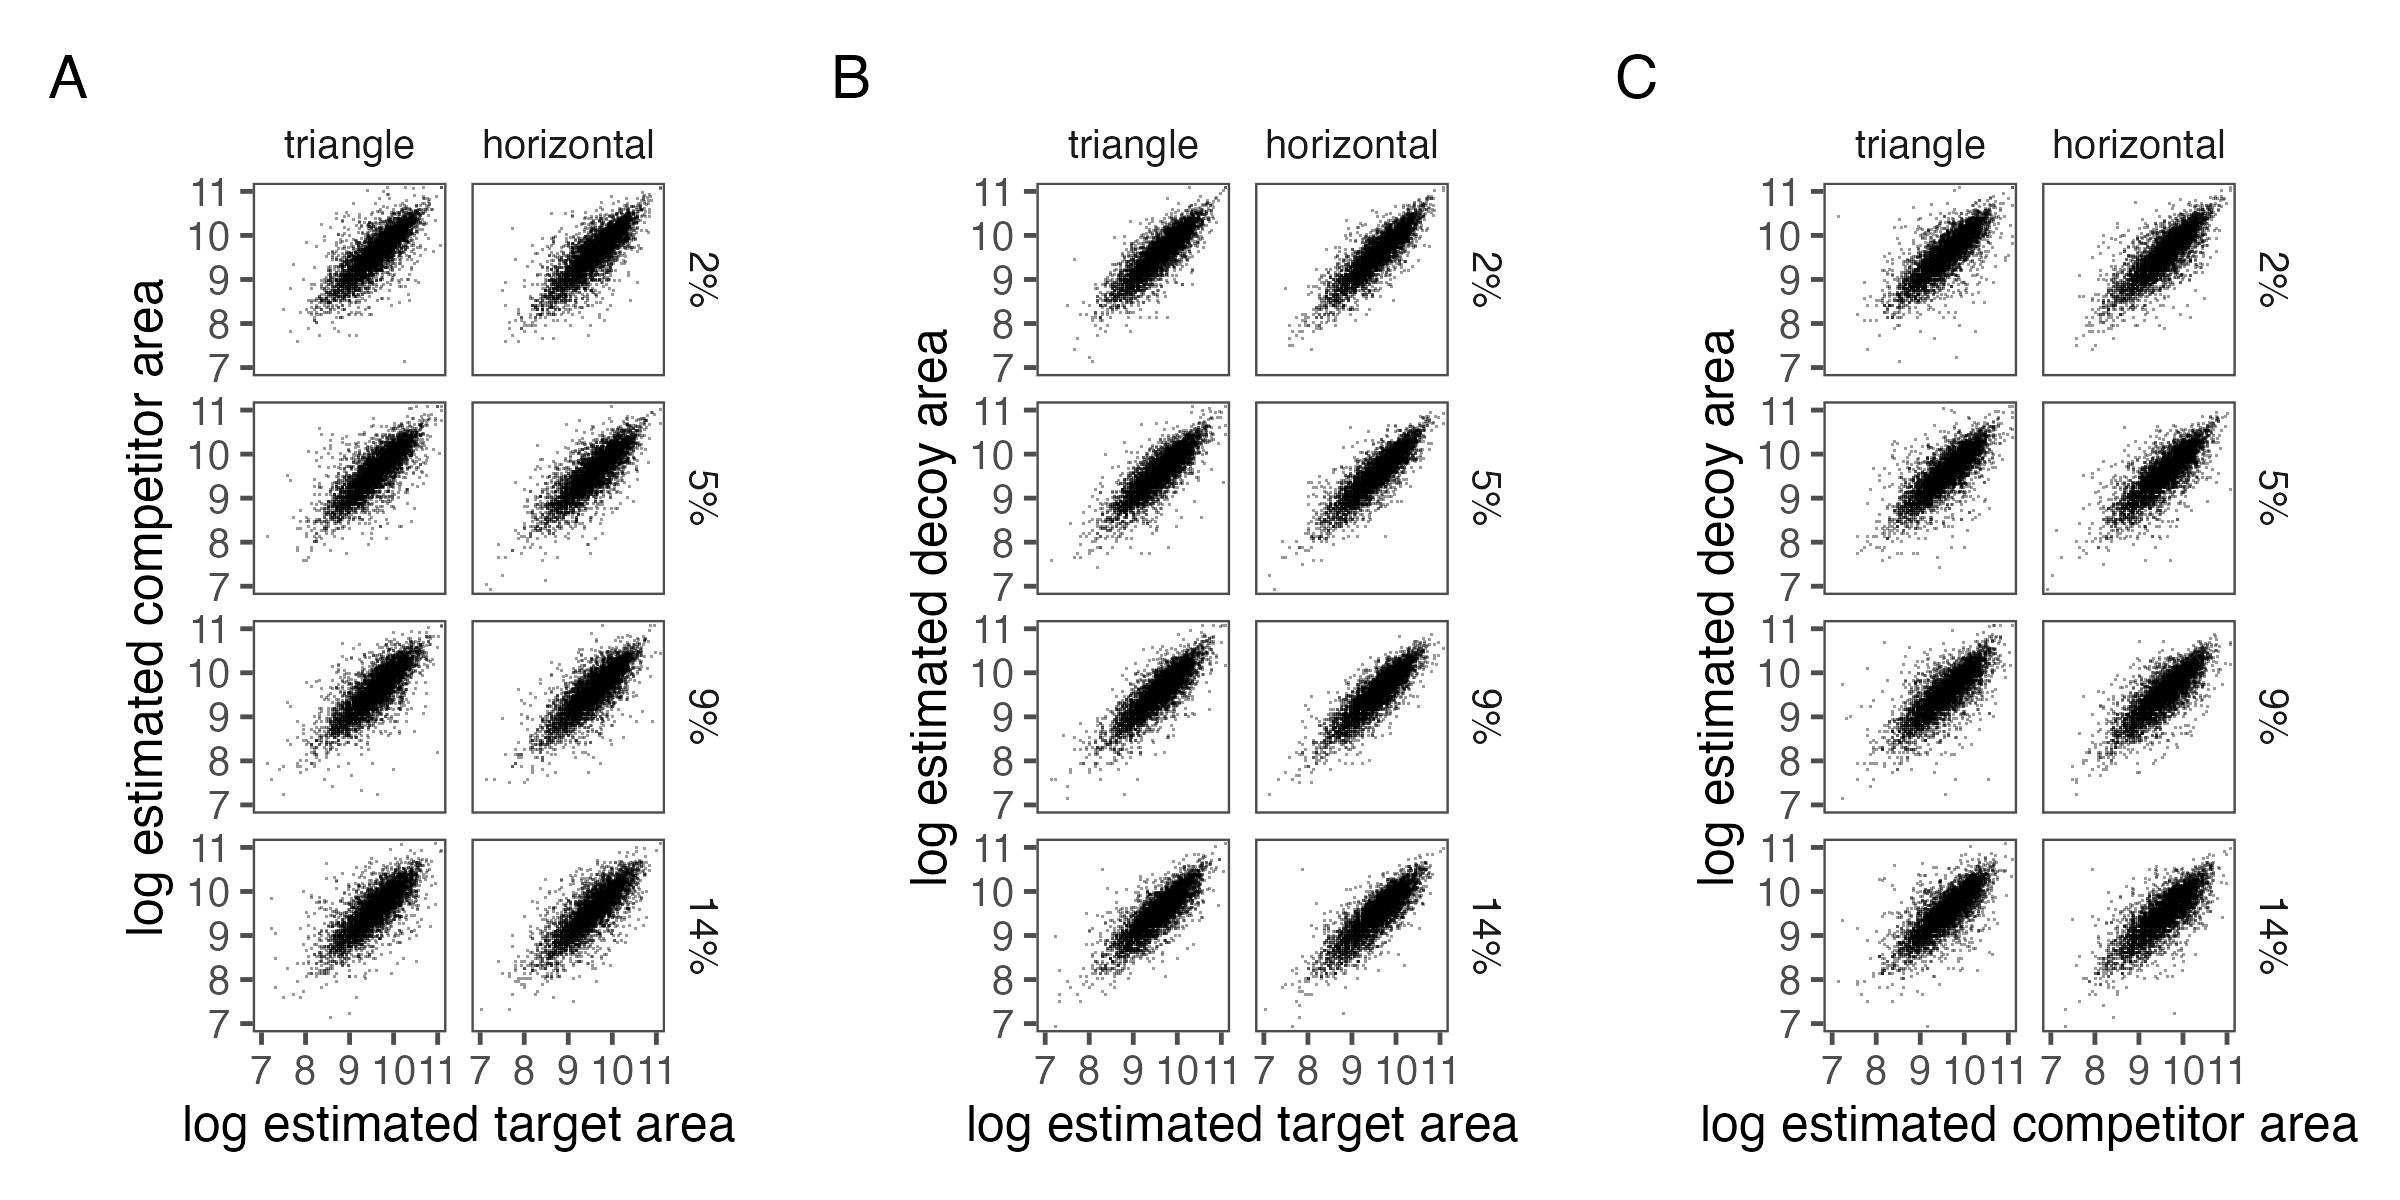
\includegraphics[width=\textwidth]{figures/circleAreaPhase_cor_plot_all_no_outliers.jpg}
   \caption{Scatterplots of target-competitor (A), target-decoy (B), and competitor-decoy (C) correlations, split by display condition and TDD.}
   \label{fig:raw_cors}
\end{figure}

Computing raw correlations, without accounting for subject and trial-level differences, will grossly inflate the size of these correlations. Moreover, any differences between, say, $\rho_{TD}$ and $\rho_{CD}$ are bound to be small. I used Bayesian hierarchical modeling to estimate the parameters of a multivariate normal distribution (as outlined in the introduction), with parameters $\mathbf{\mu}$ and $\mathbf{\sigma}$. I present the details of the model in Appendix XXX but present the main results below.

I assume that, for participant $i$, on each critical trial $j$, the perceived target, competitor, and decoy areas are sampled from a multivariate normal distribution with mean vector $\mu_{ij}$ and variance-covariance matrix $\mathbf{\Sigma}$. 

As discussed in the Introduction, I decompose sigma into the $S\mathbf{\Omega}S$, where the diagonal elements of $S$ are population standard deviations and the off diagonal elements are 0. 

I again employed Bayesian hierarchical modeling to estimate $\mathbf{\mu}$ and $\mathbf{\Omega}$. I focus on our estimates of these parameters in the main text and discuss the details of the modeling in Appendix XXX. 

I show mean estimates of $\mathbf{\mu}$ in Figure \ref{fig:e2mu} and show estimates of $\mathbf{\Omega}$ in Figure \ref{fig:omega}. In both conditions, $\rho_{TD}$ is larger than both $\rho_{CD}$ and $\rho_{TC}$, while $\rho_{CD}$ and $\rho_{TC}$ do not differ from each other. 

\begin{figure}
   \caption{Placeholder for $\mathbf{\mu}$ estimates.}
   \label{fig:e2mu}
\end{figure}

\begin{figure}
   \includegraphics[width=\textwidth]{figures/cor_intervals_plot.jpeg}
   \caption{Posterior estimates of $\Omega$ across display conditions. Inner, thick lines show $95\%$ HDIs. Outer lines show the full range of the posterior. Dots indicate means. Figure is a place holder - will show both display conditions and remove the extra whitespace.}
   \label{fig:omega}
\end{figure}

\subsubsubsection{Choice Results}

I present mean choice proportions across display conditions and TDD in figure \ref{fig:e2_choiceprops}. I replicate the qualitative results of \textcite{spektorWhenGoodLooks2018b}. At low levels of TDD, I find a repulsion effect in both display conditions. At higher levels of TDD, I either find a null effect (triangle condition) or an attraction effect (horizontal condition). 

To ensure that this result is not an artifact of averaging across choice sets, I present mean changes in choice proportion for the options $w$ and $h$ across the two choice sets $[w,h,d_{w}]$ and $[w,h,d_{h}]$ (see \ref{fig:e2_choicedeltas}). These results also show that low levels of TDD create a repulsion effect, while higher levels create a null or attraction effect. See Appendix XXX for inferential statistics that support these conclusions.

\begin{figure}
   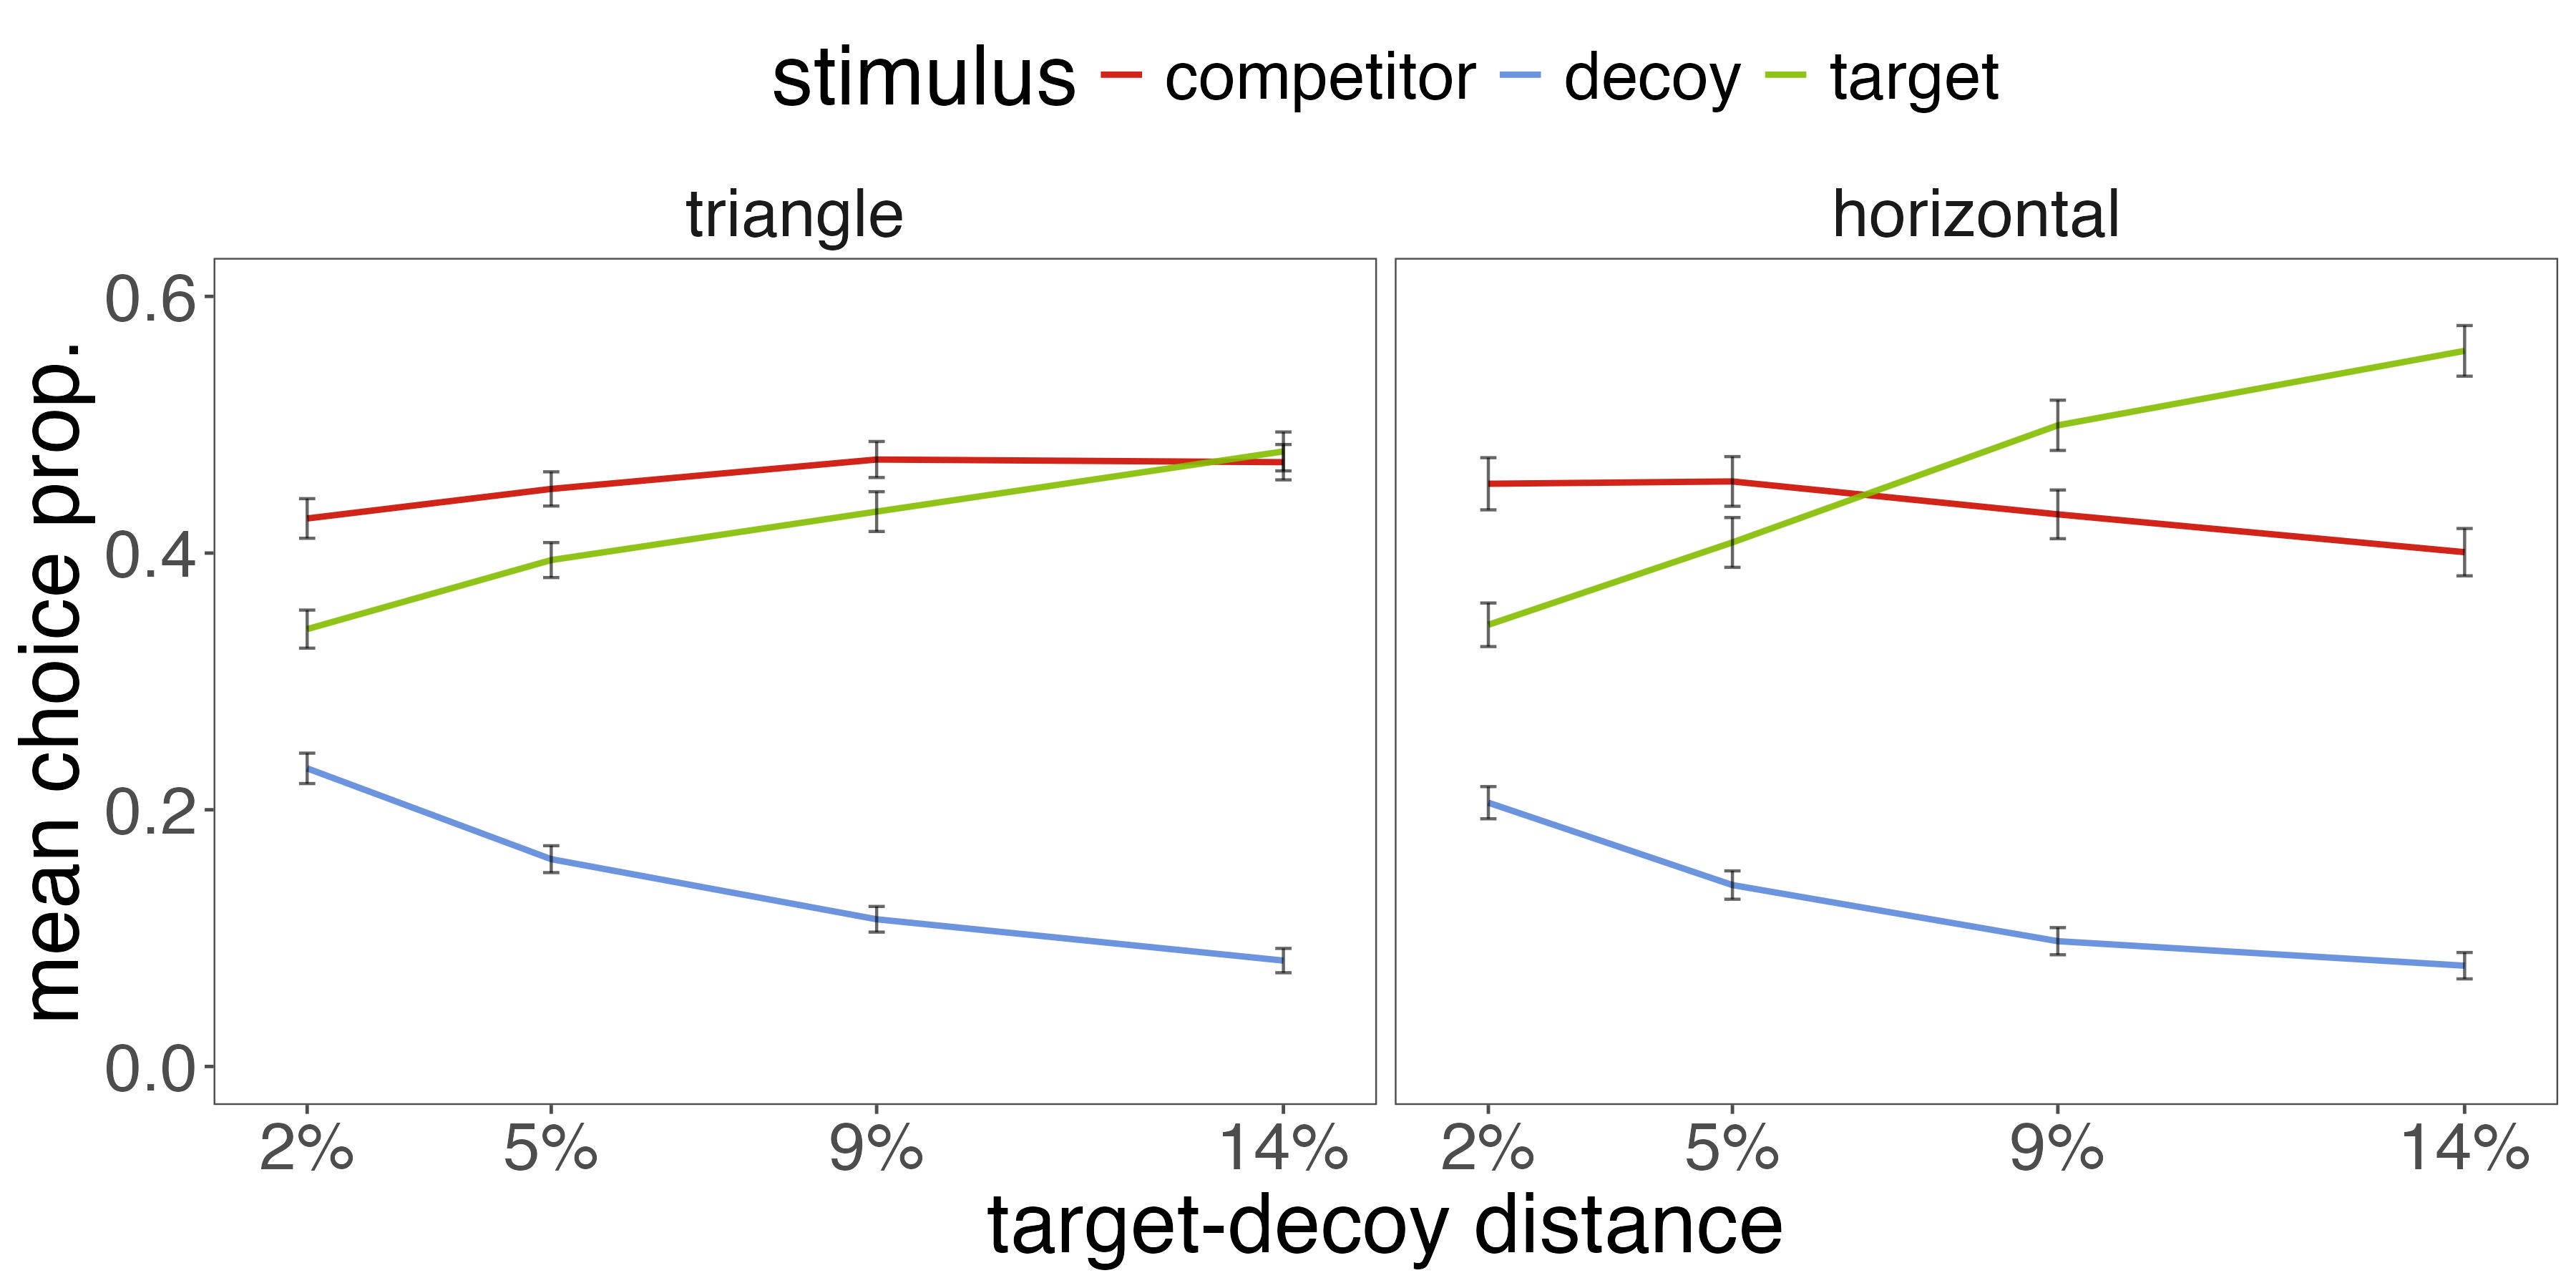
\includegraphics[width=\textwidth]{figures/choicePhase_att_trials_mean_choice_props_collapsed.jpg}
   \caption{Mean choice proportions for target, competitor, and decoy options, by TDD and display condition. THIS FIGURE IS A PLACEHOLDER. WILL CHANGE WITH HDIs FROM STAT. MODEL.}
   \label{fig:e2_choiceprops}
\end{figure}

\begin{figure}
   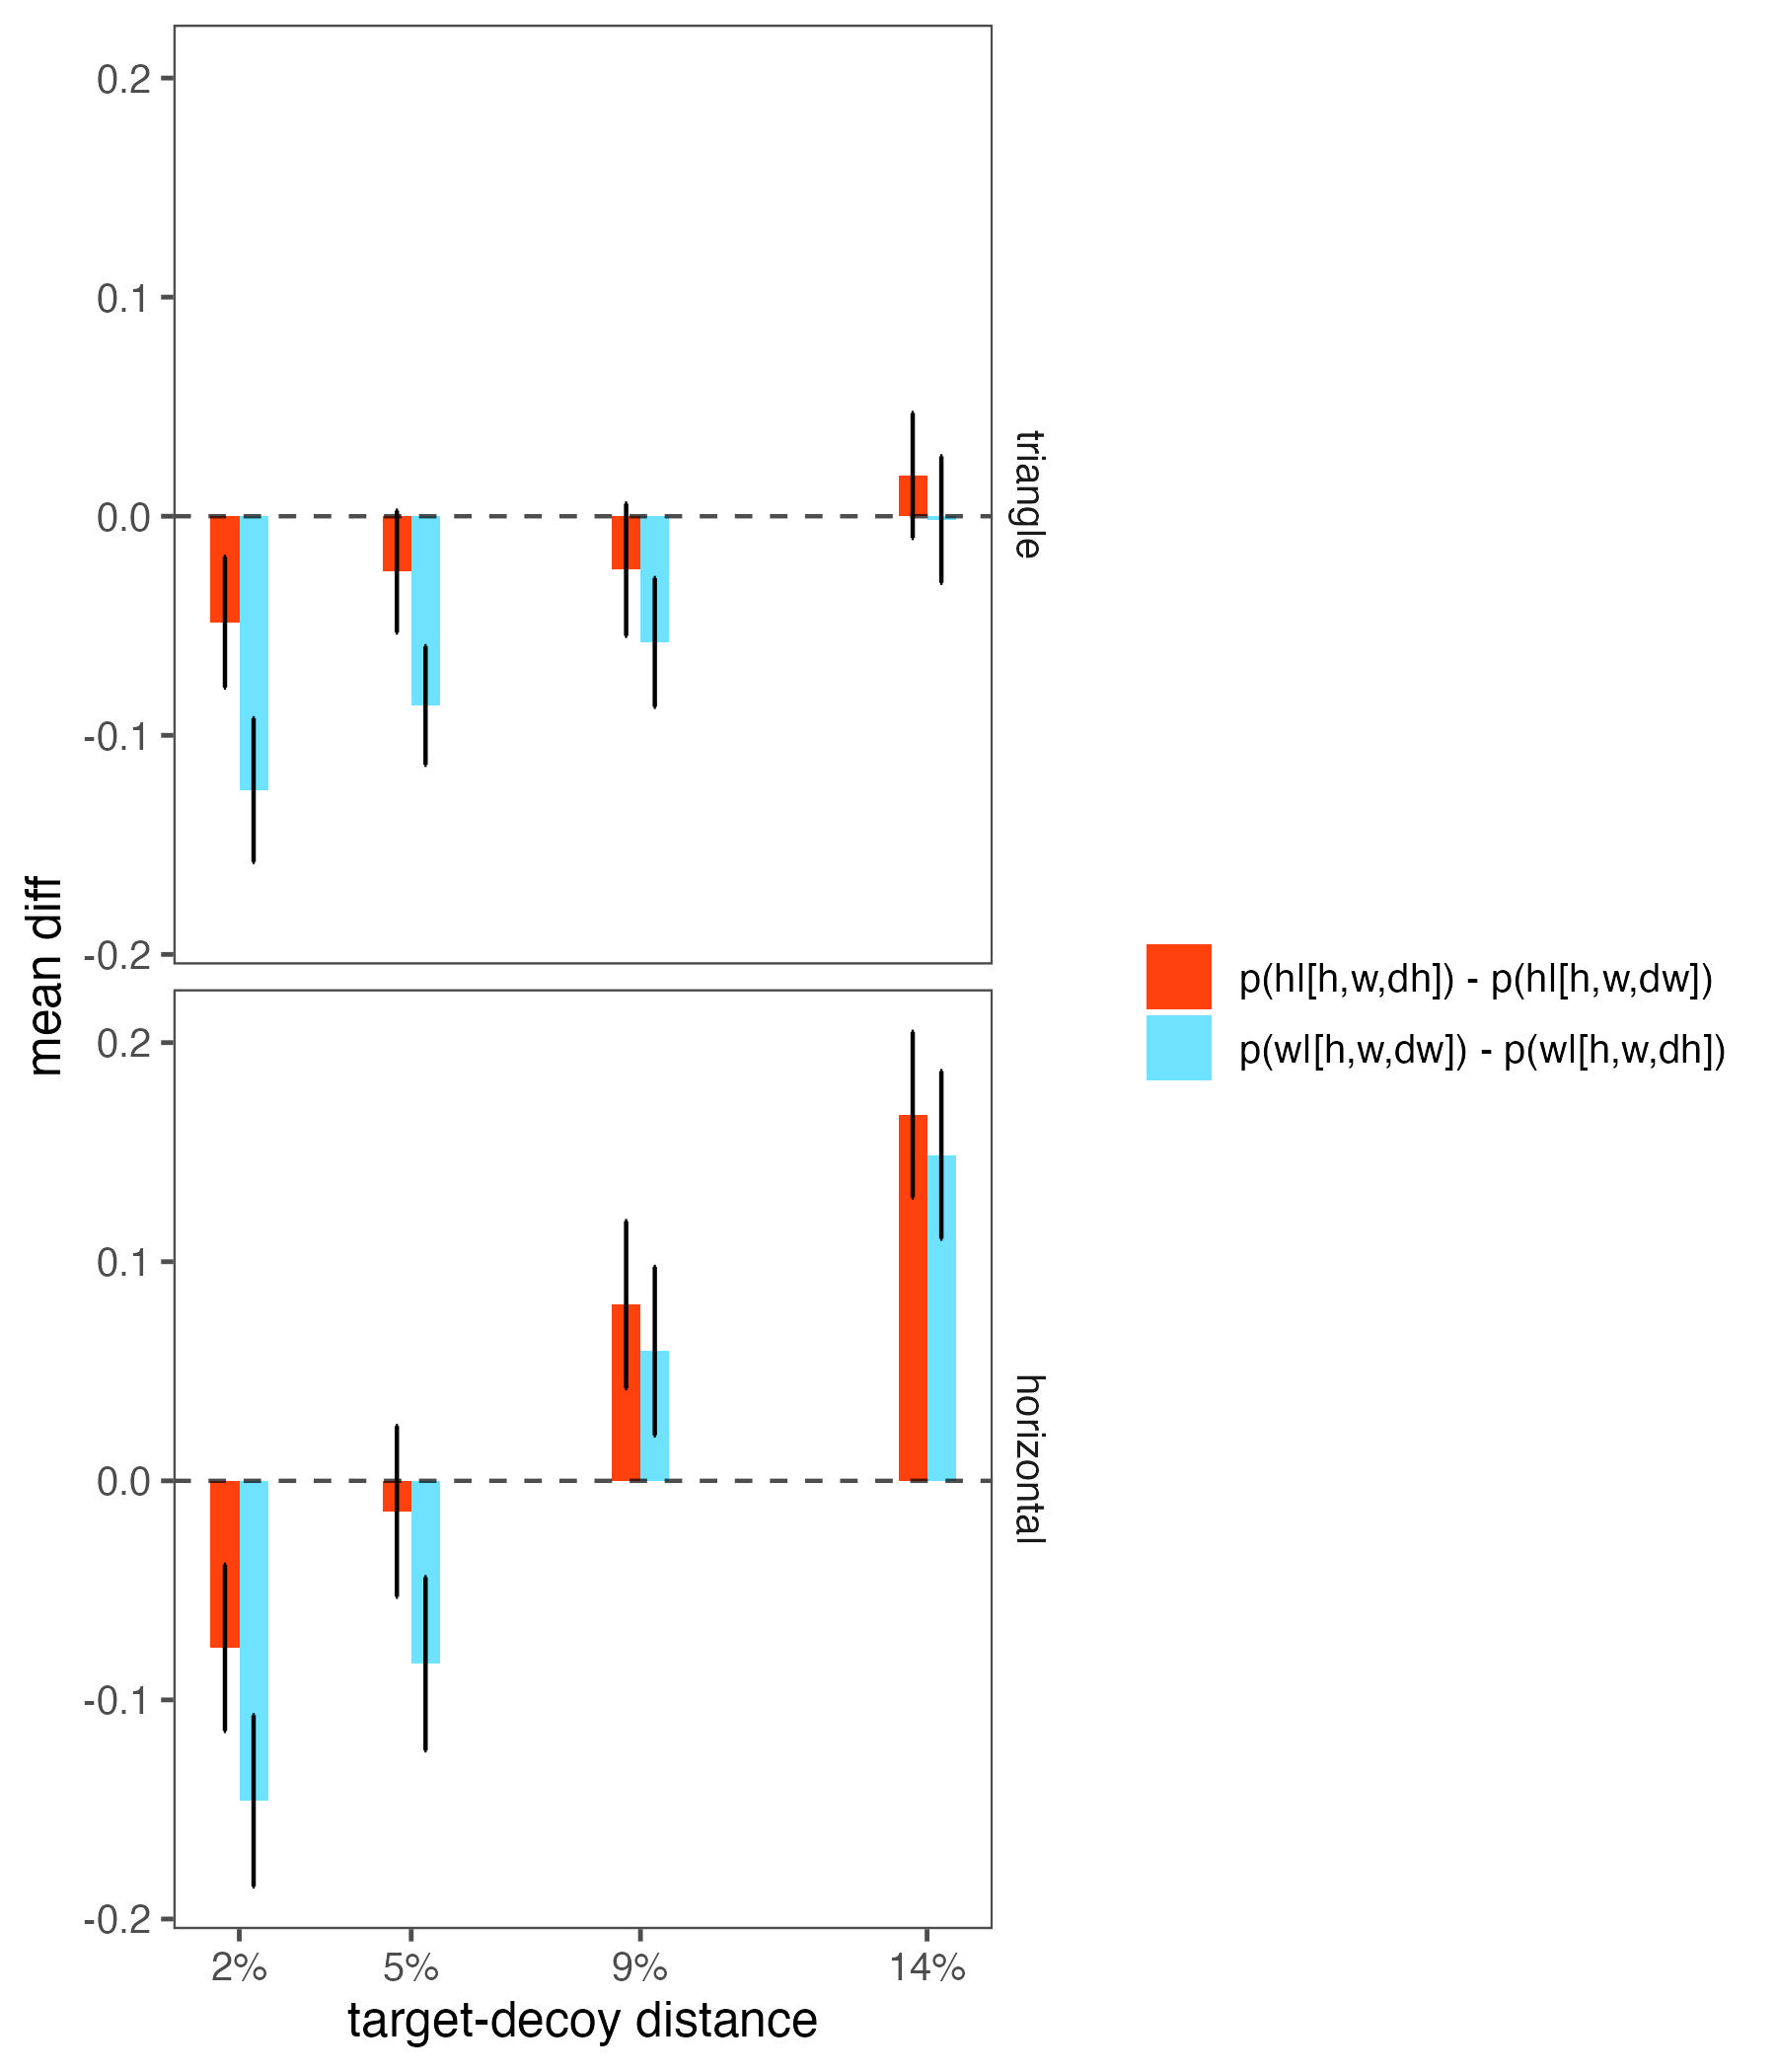
\includegraphics[width=\textwidth]{figures/choicePhase_delta_means.jpeg}
   \caption{Mean changes in choice proportions across choice sets. FIGURE IS ALSO A PLACEHOLDER}
   \label{e2_choicedeltas}
\end{figure}

\subsubsubsection{Model Simulations}
After estimating the parameters of the perceptual model and analyzing the choice data, I sought to test whether the model can predict the choice data. Though I showed in the introduction that this is possible, it was an open question whether the parameters estimated from actual data would produce qualitatively interesting predictions.

I used mean estimates of $\mathbf{\mu}$ and $\mathbf{\Sigma}$ (see Appendix XXX) to generate predictions at each level of TDD in both display conditions. I present the predictions in Figure \ref{fig:e2_model_preds}. 

Given the estimated parameters, the model is able to produce a repulsion effect, but not an attraction effect. This aligns with our predictions from the introduction; the repulsion effect, at least in some forms, can be generated by a higher correlation between target and decoy stimuli compared to target-competitor and competitor-decoy pairs.

\subsection{Discussion}

The results of Experiments 1 and 2 show that participants are not always able to discriminate the decoy from the target and the competitor, and, that target-decoy perceptions appeared to be correlated. The observed correlations can, in turn, naturally produce the repulsion effect but not the attraction effect. 

\chapter{Extending a Perceptual Model to Best-Worst Choice}

\section{Introduction}

In Chapters 1 and 2, I presented a model of perceptual choice and showed it can systematically predict the repulsion effect, but not the attraction effect. In this chapter, I test another prediction of the model while demonstrating an important empirical result in another domain: best-worst choice.

\subsection{Introducing Best-Worst Choice}

Best-worst choice (also known as best-worst scaling) is an experimental paradigm where participants select their most and least preferred options from a choice set. Originally proposed by \textcite{finn1992determining}, best-worst choice is widely used in a number of applied fields, such as transportation \parencite{beck2016best} and healthcare economics \parencite{cheung2016using,flynn2007best}. One key advantage here, when compared to traditional discrete choice research, is that researchers can use best-worst choices to gain information about participants' ranking of options while never requiring them to complete a full ranking task, which may be quite difficult \parencite{marleyProbabilisticModelsBest2005}.

In addition to the empirical applications, researchers have developed theoretical results on best-worst choice, with many models relating best-worst choices to an underlying utility function. \textcite{marleyProbabilisticModelsBest2005} developed a class of models known as "maxdiff" (maximum difference) models of best-worst choice\footnote{Note that the term maxdiff is sometimes erroneously used to refer to best-worst experiments in the generic sense. Following \textcite{marleyProbabilisticModelsBest2005}, I use maxdiff to refer to a specific class and parameterization of choice model.}. According to the maxdiff model, given choice set $K$, the probability of selecting option $x$ as best and option $y$ as worst (where $x \neq y$) is defined\parencite{hawkinsIntegratingCognitiveProcess2014a}:

\begin{equation}
   BW_{K}(x,y)=\frac{e^[u_{x}-u_{y}]}{\sum_{\substack{{p,q}\in K\\p \neq q} e^[u_{p}-u_{q}]}}
   \ref{maxdiff_equation}
\end{equation}

where $u_{i}$ is the utility of option $i$. This model proposes a single utility function that determines best and worst choices. Specifically, it proposes that best choice probabilities are an increasing function of $u$, while worst choice probabilities are a decreasing function of $u$. The use of the exponential function means that the maxdiff model is another form of the widely used multinomial logit (MNL) choice model \parencite{hausman1984specification}. Furthermore, so long as $u$ does not vary based on choice set, the maxdiff model predicts a monotonic relationship between best choice probabilities and worst choice probabilities.

There are many variations on this model \parencite{marleyProbabilisticModelsBest2005a,marleyProbabilisticModelsSetdependent2008,marleyModelsBestWorst2012,flynnBestWorstScaling2007,flynn2014best}, though the maxdiff model remains the dominant model for analyzing best-worst choice data.

Researchers have explored whether this monotonicity holds empirically. \textcite{hawkinsIntegratingCognitiveProcess2014a} examined both preferential and perceptual best-worst choice data using response time modeling. They used the linear ballistic accumulator model (LBA) \textcite{brownSimplestCompleteModel2008b}, which casts the decision process as a race between "accumulators" towards a threshold, where the average accumulation across trials is captured by the drift rate parameter. Modeling datasets containing both preferential and perceptual best-worst choice data, they were able to successfully account for choice data by assuming a parallel race between "best" and "worst" accumulators for each option. Furthermore, they showed that the utility values estimated for each option using a MNL model were positively linearly related to the log drift rate values from the LBA, suggesting an underlying utility representation that captures choices. 

In a follow-up \textcite{hawkinsBestTimesWorst2014} found that, collapsing across choice sets, best-choice probabilities are (negatively) monotonically related to worst-choice probabilities. They also showed that, using the parallel best-worst LBA as a model, the drift rate parameter for worst choice can be parameterized as the reciprocal of the best choice drift rate. Formally, if $d_{b}(i)$ is the drift rate for selecting option $i$ as best, then $d_{w}(i)=1/d_{b}(i)$, where $d_{w}(i)$ is option $i$'s drift rate for best choices. 

We can think of the parallel best-worst LBA as a process implementation of the maxdiff model \parencite{hawkinsIntegratingCognitiveProcess2014a}, which proposes set independence. While researchers have proposed models that allow set dependence \parencite{marleyProbabilisticModelsSetdependent2008}, these models still predict a monotonic relationship between best and worst choices. 

It is not always the case, however, that a single latent variable (i.e., utility) underlies choices. Indeed, as I show below, the model from Chapters 1 and 2 predicts, under certain conditions, a dissociation between best and worst choices.

\subsection{Model Predicted Dissociations Between Best Choices and Worst Choices}

Let $K$ be a choice set consistings of options $T$, $C$, and $D$ (i.e., target, competitor, and decoy). As in Experiments 1 and 2, these are rectangles in a perceptual choice experiment. As above, I asssume that on each trial $i$ with choice set $K$, The perception $\mathbf{X_i}$ of all 3 stimuli is sampled from a multivariate Gaussian distribution with a mean vector $\mathbf{\mu}$ and variance-covariance matrix $\mathbf{\Sigma}$:

\begin{align}
   \mathbf{X_{i}}\sim\mathcal{N}(\mathbf{\mu},\mathbf{\Sigma})
   \label{eqn:mvnorm}
\end{align}

$\mu$ and $\Sigma$ are parameterized the same as in Chapters 1 and 2. 

In this chapter, I apply the model to best worst choice by assuming that, given a vector $X_{i}$ of perceived areas on trial $i$ with set $K$, the probability a participant selects stimulus $i$ is as best is:

\begin{align}
   P(i|K)=P(X_{i}>X_{j}, j \in K, i \neq j)
   \label{eqn:bchoice1}
\end{align}

while the probability of selecting stimulus $k$ as worst (where $i \neq k$) is:

\begin{align}
   P(k|K)=P(X_{k}<X_{j}, j \in K, k \neq j)
   \label{eqn:wchoice1}
\end{align}

As it happens, the correlations (i.e., $\Omega$) estimated from Experiment 2 predict that, in a best-worst choice paradigm, best and worst choice probabilities are non-monotonically related. I demonstrate this using simulations.

To simulate best-worst choice, I simply used the mean parameters ($\mu$ and $\Sigma$) estimated from Experiment 2\footnote{I used only those estimated from the triangle condition (See Experiment 2).} and simulated a large ($N=10000$) number of choice trials. I collapse over choice set (as in previous reported simulations) and focus on target, competitor, and decoy choice proportions at each level of TDD. I show these results in figure \ref{fig:bw_sim}, in a state-trace plot \parencite{newell2008dimensions}. State-trace analyses plot the values of two dependent variables against each other for a particular experimental condition. State-trace analysis can be controversial \parencite{ashby2019state,ashby2022state,stephens2020state}, and statistical inference on state-trace data is not straightforward \parencite{sadil2018hierarchical,davis2016bayes}. In principle, however, if the analyst can reliably conclude that the data points do not fall on a single curve, they conclude that the data vary on at least $2$ dimensions.

\begin{figure}
   \caption{Best-worst choice simulations. Each row is a different TDD value from Experiment 2.}
   \label{fig:bw_sim}
\end{figure}

The model, conditioned on the estimated parameters, predicts an interesting result. Although the competitor is most frequently chosen as best, due to the repulsion effect from Experiment 2 and from \textcite{spektorWhenGoodLooks2018b}, it is not, however, least frequently chosen as worst. Specifically, $B_{C}>B_{T}>B_{D}$, while $W_{T}<W_{C}<W_{D}$, where $B_{i}$ and $W_{i}$ are the probabilities that option $i$ is chosen as best and worst, respectively.

The reason for this prediction is that because $\rho_{TD}>\rho_{CD}\approx\rho_{TC}$, on the (relatively few) trials where $X_{D}$ is largest, it is more likely that $X_{D}>X_{T}>X_{C}$ than $X_{D}>X_{C}>X_{T}$. In other words, the high $\rho_{TD}$ value "pulls up" the target more than the competitor.

This dissociation is subtle, and the predicted effect size is small. Indeed, all predicted $W_{C}-W_{T}$ probabilities were $<.05$. However, In Experiment 3, I show the empirical and modeling results from a best-worst choice experiment designed to test this prediction. I show that the dissociation between best and worst choices does indeed occur, and the maxdiff model cannot account for these results.

\section{Experiment 3}

%% End of body
%%%%%%%%%%%%%%%%%%%%%%%%%%%%%%%%%%%%%%%%%%%%%%%%%%%%%%%%%%%%%%%%%%%%%%%%%%%%%%%

\appendix
\chapter{Experiment 1: Bayesian Logistic Regression Model of 2AFC Discriminability}
...
\chapter{Experiment 2: Bayesian Hierarchical Modeling of Circle Estimation of Data}
...

%%
%% Beginning of back matter
\backmatter  %% <--- mandatory

%%
%% Idon't support endnotes

%%
%% A bibliography is required.
\interlinepenalty=10000  % prevent split bibliography entries
\printbibliography
\end{document}

%%% Local Variables: 
%%% mode: latex
%%% TeX-master: t
%%% End: 
